\documentclass[conference]{IEEEtran}
\IEEEoverridecommandlockouts

\usepackage[T1]{fontenc}
\usepackage{cite}
\usepackage{amsmath,amssymb}
\usepackage{graphicx}
\usepackage{booktabs}
\usepackage{multirow}
\usepackage{xcolor}
\usepackage{array}
\usepackage[hidelinks]{hyperref}
\usepackage{url}

\graphicspath{{figures/}}
\renewcommand{\arraystretch}{1.12}
% let figures sit closer to the text that cites them
\renewcommand{\topfraction}{0.9}
\renewcommand{\dbltopfraction}{0.9}
\renewcommand{\bottomfraction}{0.6}
\renewcommand{\textfraction}{0.1}
\renewcommand{\floatpagefraction}{0.75}
\renewcommand{\dblfloatpagefraction}{0.75}
\setcounter{topnumber}{3}
\setcounter{dbltopnumber}{2}
\setcounter{totalnumber}{5}

\begin{document}

\title{NOVA-Net: Predicting the Processing Level of Packaged Foods from Nutrition, Ingredients and Categories with Open Food Facts}

\author{
\IEEEauthorblockN{Omar Ahmed Elwekeil}
\IEEEauthorblockA{\textit{Artificial Intelligence Program} \\
\textit{Egypt-Japan University of Science and Technology}\\
Alexandria, Egypt \\
ID: 320230172}
\and
\IEEEauthorblockN{Ahmed Abdelmaksoud}
\IEEEauthorblockA{\textit{Artificial Intelligence Program} \\
\textit{Egypt-Japan University of Science and Technology}\\
Alexandria, Egypt \\
ID: 320230212}
}

\maketitle

\begin{abstract}
Ultra-processed foods are associated with obesity, type 2 diabetes and cardiovascular disease, yet most packaged products carry no processing label. The NOVA system rates processing from 1 (unprocessed) to 4 (ultra-processed), but only 23.3\% of the 4.8 million products in the Open Food Facts database have a NOVA group. NOVA-Net predicts a product's NOVA group from its nutrition facts, ingredient text and category tags. We study the 993,157 United States products in the database, of which 388,530 are labeled. The data are difficult: the classes are imbalanced 28:1, ingredient-derived inputs are missing for 88\% of unlabeled products, up to 4\% of nutrient values are physically impossible, and a copy of the label is hidden inside the nested nutrient records. On a stratified sample of 120,000 labeled products we build an 84-feature representation and compare eleven dimensionality-reduction methods (PCA, LDA, SVD, Kernel PCA, SNE, t-SNE, UMAP, metric and non-metric MDS, Isomap, LLE), K-Means clustering, twelve feature-selection methods (filter, wrapper, embedded and two metaheuristics) and five classifiers. LDA is the only 2-D projection that separates the classes (kNN accuracy 79.5\%, K-Means ARI 0.42). Feature selection can remove up to 40 features at a cost of at most 0.013 macro-F1. A Random Forest reaches 93.8\% accuracy, 0.910 macro-F1 and 0.990 ROC-AUC on a held-out 20\% test set, and 78\% of its errors are between neighbouring NOVA groups. Ablations show that ingredient text carries most of the signal (0.846 macro-F1 alone) while nutrients alone reach 0.696. We discuss why Open Food Facts' rule-based labels shape these results and what they imply for labeling the products that lack a NOVA group.
\end{abstract}

\begin{IEEEkeywords}
food processing, NOVA classification, ultra-processed food, Open Food Facts, dimensionality reduction, feature selection, genetic algorithm, particle swarm optimisation, random forest, class imbalance, data leakage
\end{IEEEkeywords}

%% =========================================================
\section{Introduction}

Diets high in ultra-processed food are linked to obesity, type 2 diabetes, cardiovascular disease, depression and all-cause mortality~\cite{lane2024bmj}. The NOVA classification~\cite{monteiro2019nova} groups foods by the extent and purpose of industrial processing into four classes: (1) unprocessed or minimally processed foods such as fruit, vegetables, plain milk and eggs; (2) processed culinary ingredients such as oils, butter, sugar and salt; (3) processed foods such as canned vegetables, cheese and simple breads; and (4) ultra-processed foods, industrial formulations such as soft drinks, packaged snacks and reconstituted meat that typically contain additives with cosmetic functions. Unlike nutrient-based scores, NOVA does not appear on food packages, so consumers, researchers and public-health agencies cannot easily tell how processed a product is.

Open Food Facts (OFF)~\cite{off} is a non-profit, crowd-sourced database of packaged foods. It assigns a NOVA group to products for which it has enough information, but in the current export only 1,120,043 of 4,807,583 products (23.3\%) have one. A model that predicts NOVA from whatever information \emph{is} available could label the remaining products and support large-scale dietary research and consumer tools.

NOVA-Net is a course project that builds such a model. Its first phase, reported here, has two parts. The first is a full exploratory analysis of the United States subset of OFF, which shows how difficult the data are. The second applies and compares the main families of techniques from the course: linear and nonlinear dimensionality reduction, clustering, feature selection, and supervised classification with a complete evaluation.

Our contributions are:
\begin{itemize}
    \item A reproducible pipeline that loads the 7.7\,GB Parquet export with DuckDB, flattens nested nutrient records, removes target leakage and impossible values, and produces a cleaned table of 993,157 US products.
    \item A quantitative study of the data's difficulties: 28:1 class imbalance, missing values, crowd-entry errors, noisy text, correlated nutrients, high-cardinality tags and sparse, high-dimensional text.
    \item A comparison of eleven dimensionality-reduction methods, including an implementation of the original SNE, scored by class separation, kNN accuracy, trustworthiness and agreement of K-Means clusters with the labels.
    \item A comparison of twelve feature-selection methods (filter, wrapper, embedded, genetic algorithm and binary particle swarm optimisation) under one common evaluator.
    \item Five classifiers trained on three feature sets and evaluated with accuracy, error rate, precision, recall, F1, ROC-AUC, confusion matrices, 5-fold cross-validation, over- and underfitting diagnostics, and ablations by feature group, compared with four published NOVA classifiers.
\end{itemize}

Section~\ref{sec:related} reviews related work. Section~\ref{sec:data} describes the dataset and Section~\ref{sec:method} the methodology. Section~\ref{sec:eda} reports the exploratory analysis, Section~\ref{sec:reduction} the reduction and clustering results, Section~\ref{sec:selection} feature selection, and Section~\ref{sec:models} the classifiers and their evaluation. Section~\ref{sec:discussion} interprets the results and Section~\ref{sec:conclusion} concludes.

%% =========================================================
\section{Related Work}
\label{sec:related}

\subsection{The NOVA classification and its automation}
Monteiro \emph{et al.}~\cite{monteiro2019nova} define the NOVA groups and the ``markers'' of ultra-processing: cosmetic additives (colours, flavours, emulsifiers, sweeteners) and industrial ingredients rarely used in home cooking (hydrolysed proteins, maltodextrin, invert sugar). Assigning NOVA by hand requires reading the full ingredient list and knowing how the product was made, which does not scale to millions of products. OFF implements a rule-based version of these criteria~\cite{offnova}: a product starts in group~1 and moves to group 2, 3 or 4 when its categories or ingredients match marker lists. The NOVA labels in OFF are therefore themselves the output of a deterministic procedure, a fact that shapes every model trained on them (Section~\ref{sec:discussion}).

\subsection{Machine-learning prediction of NOVA}
Menichetti \emph{et al.}~\cite{menichetti2023foodprox} showed that the degree of processing can be predicted from nutrient concentrations alone. Their FoodProX random-forest model, trained on 7,253 manually classified foods from the US Food and Nutrient Database for Dietary Studies (FNDDS), reached one-vs-rest ROC-AUC between 0.963 and 0.980 per class. Arora \emph{et al.}~\cite{arora2025fndds} compared gradient-boosting models on FNDDS with 13 to 102 nutrients and reported F1 between 0.928 and 0.941. In a follow-up on OFF itself~\cite{arora2025off}, with 480,000 to 875,000 products and 7 to 44 nutrients, accuracy dropped to 0.80--0.85 and F1 to 0.79--0.84. This drop shows how much harder crowd-sourced branded-product data are than curated generic foods.

Hu \emph{et al.}~\cite{hu2023nutrients} instead classified products from their ingredient text. A fine-tuned MiniLM language model trained on 18,916 manually labeled Canadian products reached 0.979 accuracy, and 0.948 on US branded foods. An XGBoost model on nutrients only reached 0.890. Their results suggest that ingredient text carries more information about processing than nutrients do, a conclusion our ablations confirm (Section~\ref{sec:ablation}).

\subsection{Dimensionality reduction and feature selection}
Linear methods such as PCA and LDA~\cite{bishop2006} project data onto directions of maximum variance or maximum class separation. Nonlinear manifold methods preserve other structure: geodesic distances (Isomap~\cite{tenenbaum2000isomap}), local linear reconstructions (LLE~\cite{roweis2000lle}), neighbour probabilities (SNE~\cite{hinton2002sne}, t-SNE~\cite{vandermaaten2008tsne}) or a fuzzy neighbour graph (UMAP~\cite{mcinnes2018umap}). Multidimensional scaling~\cite{borg2005mds} preserves pairwise distances (metric) or their rank order (non-metric). Feature-selection methods are commonly grouped into filters, wrappers and embedded methods~\cite{guyon2003}. Metaheuristics such as genetic algorithms~\cite{holland1975} and binary particle swarm optimisation~\cite{kennedy1997bpso} search the space of feature subsets directly. To our knowledge, no prior work has compared these method families on NOVA prediction.

%% =========================================================
\section{Dataset}
\label{sec:data}

We use the official OFF Parquet export hosted on Hugging Face~\cite{offhf} (file \texttt{food.parquet}, 7.7\,GB, 111 columns, Open Database License). Each row is one packaged product with its barcode, name, brand, ingredient list, nutrient table, categories, labels, additives, allergens and packaging. The target is \texttt{nova\_group} $\in \{1,2,3,4\}$.

We keep products whose \texttt{countries\_tags} list contains \texttt{en:united-states}. The US is the country with the most labeled products: 388,530 of its 993,157 products (39.1\%). The labeled products form the modelling table; the 604,627 unlabeled products are kept to study the population a model would be applied to. The export is refreshed regularly, so counts may shift slightly between downloads.

The dataset is difficult in several ways, each quantified in Section~\ref{sec:eda}. The classes are severely imbalanced. Many fields are missing, and missingness differs sharply between labeled and unlabeled products. Crowd-entered values contain physically impossible numbers. The ingredient text is noisy and duplicated. Nutrients are stored as a nested list. Categories and brands have thousands of distinct values. Text features are sparse and high-dimensional. Finally, the classes overlap in nutrient space.

%% =========================================================
\section{Methodology}
\label{sec:method}

The pipeline runs in a single Google Colab notebook. Part~A loads, cleans and explores the data; Part~B applies reduction, selection and classification.

\subsection{Loading, flattening and leakage removal}
The Parquet file is queried with DuckDB~\cite{duckdb}, which reads only the requested columns and keeps memory within a free Colab instance. Nutrients are stored as a list of records \{\textit{name}, \textit{value}, \textit{100g}, \textit{unit}, \dots\}. We pivot the nine core nutrients (energy, fat, saturated fat, carbohydrates, sugars, fiber, proteins, salt, sodium) and the most frequent others into per-100\,g columns. Multilingual fields are reduced to one string, preferring English.

Three fields copy the label: \texttt{nova\_groups}, \texttt{nova\_groups\_tags}, and a \texttt{nova-group} entry inside the nutrient list, present for 96\% of labeled products. A naive flattening of the most frequent nutrients would include this entry as a feature. All three are excluded, as is \texttt{nutrition-score-fr}, a score that OFF computes from the nutrients.

\subsection{Cleaning}
Impossible nutrient values are set to missing rather than removing the product, so its text and categories remain usable. A value is impossible if it is negative, exceeds 100\,g per 100\,g, or exceeds 900\,kcal (3,800\,kJ). Saturated fat above total fat and sugars above carbohydrates (with a 0.5\,g tolerance) are also removed. Fat, carbohydrates and proteins are all removed when their sum exceeds 105\,g.

\subsection{Sampling, split and feature matrix}
For Part~B we draw a stratified sample of 120,000 labeled products, which keeps the class shares of the full table. We then split it 80/20 into 96,000 training and 24,000 test products, also stratified. The split is made first. Every step that learns from data (imputation medians, frequent tags, TF-IDF and SVD, scaling, reduction and selection) is fitted on the training part only, so the test set is used only for the final evaluation.

The feature matrix has 84 columns:
\begin{itemize}
    \item \textbf{Nutrients (17):} the eight core nutrients (sodium dropped as a duplicate of salt) and nine minor nutrients, transformed with $\log(1+x)$ to reduce their heavy right tails and imputed with the training median.
    \item \textbf{Counts (3):} ingredient count, additive count and number of words in the ingredient text, also log-transformed.
    \item \textbf{Missing-value flags (9):} one per core nutrient and one for missing ingredient text.
    \item \textbf{Tags (35):} multi-hot indicators of the 25 most frequent category tags and 10 most frequent label tags, with placeholders such as \texttt{en:undefined} removed.
    \item \textbf{Text (20):} the first 20 components of a truncated SVD of TF-IDF vectors (1--2-grams, minimum document frequency 5, sublinear term frequency) computed on the ingredient text.
\end{itemize}
All columns are standardised to zero mean and unit variance.

\subsection{Linear dimensionality reduction}
\textbf{PCA} finds orthonormal directions $w$ that maximise the variance of the projected data. They are the eigenvectors of the covariance matrix:
\begin{equation}
\Sigma = \tfrac{1}{n} X^\top X, \qquad \Sigma w_k = \lambda_k w_k,
\end{equation}
where $X$ is centred and $\lambda_k$ is the variance along $w_k$.

\textbf{LDA} uses the labels. It finds at most $C-1 = 3$ directions that maximise between-class scatter $S_B$ relative to within-class scatter $S_W$:
\begin{equation}
W^\ast = \arg\max_W \frac{\left| W^\top S_B W \right|}{\left| W^\top S_W W \right|}.
\end{equation}

\textbf{Truncated SVD} factorises the data matrix without centring, $X \approx U_k \Sigma_k V_k^\top$, which is why it also applies to sparse TF-IDF matrices.

\subsection{Nonlinear dimensionality reduction}
\textbf{Kernel PCA} performs PCA in the feature space of a kernel. We use the RBF kernel $k(x,x') = \exp(-\gamma \|x-x'\|^2)$ with $\gamma = 1/p$, where $p$ is the number of features.

\textbf{SNE}~\cite{hinton2002sne} converts distances into conditional probabilities. In the original space, $x_j$ is a neighbour of $x_i$ with probability
\begin{equation}
p_{j|i} = \frac{\exp(-\|x_i - x_j\|^2 / 2\sigma_i^2)}{\sum_{k \neq i} \exp(-\|x_i - x_k\|^2 / 2\sigma_i^2)},
\end{equation}
where $\sigma_i$ is set by binary search so that the perplexity $2^{H(P_i)}$ equals 30. In the 2-D map, $q_{j|i}$ uses a Gaussian with fixed variance $\tfrac{1}{2}$. SNE minimises $C = \sum_i \mathrm{KL}(P_i \,\|\, Q_i)$ by gradient descent with momentum, using the gradient
\begin{equation}
\frac{\partial C}{\partial y_i} = 2 \sum_j \left(p_{j|i} - q_{j|i} + p_{i|j} - q_{i|j}\right)(y_i - y_j).
\end{equation}
SNE is not available in scikit-learn, so we implemented it directly and verified the gradient against a numerical finite difference.

\textbf{t-SNE}~\cite{vandermaaten2008tsne} symmetrises the probabilities and replaces the 2-D Gaussian with a Student-$t$ kernel, $q_{ij} \propto (1 + \|y_i - y_j\|^2)^{-1}$. Its heavy tail relieves SNE's ``crowding problem''.

\textbf{UMAP}~\cite{mcinnes2018umap} builds a fuzzy $k$-nearest-neighbour graph (15 neighbours) and lays it out in 2-D by minimising a cross-entropy between edge weights (minimum distance 0.1).

\textbf{Metric MDS} minimises the stress between original distances $d_{ij}$ and embedded distances $\hat d_{ij}$ with the SMACOF algorithm~\cite{borg2005mds}:
\begin{equation}
\mathrm{Stress} = \sum_{i<j} \left(d_{ij} - \hat d_{ij}\right)^2.
\end{equation}
\textbf{Non-metric MDS} preserves only the rank order of the distances, through a monotone transformation of $d_{ij}$.

\textbf{Isomap}~\cite{tenenbaum2000isomap} applies MDS to geodesic distances, i.e.\ shortest paths in a 10-nearest-neighbour graph. \textbf{LLE}~\cite{roweis2000lle} writes each point as a weighted combination of its 12 nearest neighbours and finds the 2-D coordinates that keep the same weights.

PCA, LDA and SVD are fitted on all 96,000 training products. Most nonlinear methods scale quadratically with the number of points, so they are fitted on a balanced sample of 2,000 training products (500 per class). MDS and SNE use a 1,000-point subset of it.

\subsection{Evaluating embeddings and clustering}
Each 2-D embedding is scored with four measures:
\begin{itemize}
    \item \textbf{Silhouette} of the true classes,
    \begin{equation}
    s = \frac{1}{N}\sum_{i=1}^{N}\frac{b_i - a_i}{\max(a_i, b_i)},
    \end{equation}
    where $a_i$ is the mean distance to points of the same class and $b_i$ the mean distance to the nearest other class.
    \item \textbf{kNN accuracy}: 5-fold cross-validated accuracy of a 10-nearest-neighbour classifier on the 2-D coordinates. Chance is 25\% on the balanced sample.
    \item \textbf{Trustworthiness}~\cite{venna2001trust}: whether a point's 10 nearest neighbours in 2-D are also near it in the original space (1 = fully preserved).
    \item \textbf{K-Means agreement}: K-Means with $k=4$ is run on the embedding, and its clusters are compared with the NOVA labels by the Adjusted Rand Index (ARI) and Normalised Mutual Information (NMI).
\end{itemize}
K-Means is also run on the original 84-dimensional features, with elbow and silhouette curves for $k=2,\dots,8$.

\subsection{Feature selection}
Each method returns a feature subset. All subsets are then scored by the same evaluator: a class-weighted Histogram Gradient Boosting classifier, 3-fold stratified cross-validated macro-F1, on 20,000 training products.

\textbf{Filter methods} rank features without a model:
\begin{itemize}
    \item variance after min-max scaling, with a threshold of 0.01;
    \item mutual information $I(X_j;Y)$, with a nearest-neighbour estimator for continuous features;
    \item the ANOVA $F$ statistic, the ratio of between-class to within-class variance;
    \item the $\chi^2$ statistic on min-max-scaled features;
    \item a correlation filter that walks features in order of mutual information and drops any feature with $|r| > 0.9$ to one already kept.
\end{itemize}
The top-$k$ filters keep $k=20$ features.

\textbf{Wrapper methods} search subsets by retraining a model. All three use a class-weighted logistic regression scored by 3-fold macro-F1 on 8,000 training products:
\begin{itemize}
    \item sequential forward selection, starting from the 30 features with the highest mutual information and adding one feature at a time;
    \item sequential backward elimination over the same 30 candidates, removing one at a time;
    \item recursive feature elimination (RFE) over all 84 features, which repeatedly removes the two with the smallest coefficients.
\end{itemize}
Each stops at 15 features.

\textbf{Embedded methods} select during training. Multinomial logistic regression with $C=0.05$ minimises the cross-entropy plus a penalty $\lambda \Omega(w)$:
\begin{itemize}
    \item L1 (Lasso), $\Omega = \|w\|_1$, sets weak weights exactly to zero;
    \item L2 (Ridge), $\Omega = \|w\|_2^2$, only shrinks them, so we keep the 20 features with the largest mean $|w|$;
    \item Elastic Net, $\Omega = \alpha\|w\|_1 + (1-\alpha)\|w\|_2^2$ with $\alpha = 0.5$, is sparse like L1 but keeps correlated groups together.
\end{itemize}

\textbf{Metaheuristics} search the space of binary masks $m \in \{0,1\}^{84}$ directly. Both maximise
\begin{equation}
f(m) = \text{macro-F1}_{\text{CV}}(X_{:,m}) - 0.02\,\frac{|m|}{p},
\end{equation}
where the score comes from the wrapper's logistic regression. The small penalty prefers smaller subsets when scores tie.
\begin{itemize}
    \item The \textbf{genetic algorithm} evolves 24 masks for 20 generations, using tournament selection (size 3), uniform crossover with probability 0.9, bit-flip mutation with probability $1/p$, and elitism of 2.
    \item \textbf{Binary PSO}~\cite{kennedy1997bpso} moves 20 particles for 15 iterations with velocity update
    \begin{equation}
    v \leftarrow w v + c_1 r_1 (p_{\text{best}} - x) + c_2 r_2 (g_{\text{best}} - x),
    \end{equation}
    where $w = 0.7$ and $c_1 = c_2 = 1.5$. A bit is then set with probability $\sigma(v)$.
\end{itemize}

\subsection{Classifiers}
Five classifiers of increasing flexibility are trained~\cite{sklearn}:
\begin{itemize}
    \item multinomial logistic regression;
    \item $k$-nearest neighbours ($k=15$);
    \item a fully grown decision tree;
    \item a random forest of 200 trees with at least two samples per leaf;
    \item histogram gradient boosting with up to 300 iterations and early stopping.
\end{itemize}
Class weights inversely proportional to class frequency are used wherever the model supports them, to counter the imbalance. Each model is trained on three feature sets: all 84 features, the best selected subset, and the 56 PCA components that keep 95\% of the variance.

\subsection{Evaluation}
On the 24,000-product test set we report:
\begin{itemize}
    \item accuracy $= (TP+TN)/N$ and error rate $= 1 - $ accuracy;
    \item per-class precision $TP/(TP+FP)$, recall $TP/(TP+FN)$ and F1 $= 2PR/(P+R)$;
    \item one-vs-rest ROC-AUC.
\end{itemize}
Macro averages treat the four classes equally, which matters under a 28:1 imbalance; weighted averages follow class sizes. We also report:
\begin{itemize}
    \item confusion matrices;
    \item 5-fold stratified cross-validation on 30,000 training products;
    \item a fit diagnosis comparing training and test macro-F1: a gap above 0.07 is read as overfitting, and both scores below 0.60 as underfitting;
    \item a learning curve for the best model;
    \item an ablation that retrains gradient boosting on single feature groups.
\end{itemize}

%% =========================================================
\section{Exploratory Analysis}
\label{sec:eda}

\subsection{Class imbalance}
Table~\ref{tab:classes} and Fig.~\ref{fig:classes} show the class distribution. NOVA~4 dominates with 70.5\% of labeled products, while NOVA~2 has only 2.5\%, an imbalance ratio of 28. A classifier that always predicts NOVA~4 would reach 70.5\% accuracy without learning anything.

\begin{table}[t]
\centering
\caption{NOVA class distribution, labeled US products}
\label{tab:classes}
\begin{tabular}{llrr}
\toprule
Group & Description & Products & Share \\
\midrule
1 & Unprocessed / minimally processed & 38,425 & 9.9\% \\
2 & Processed culinary ingredients & 9,738 & 2.5\% \\
3 & Processed foods & 66,432 & 17.1\% \\
4 & Ultra-processed foods & 273,935 & 70.5\% \\
\midrule
 & Total & 388,530 & 100\% \\
\bottomrule
\end{tabular}
\end{table}

\begin{figure}[t]
\centering
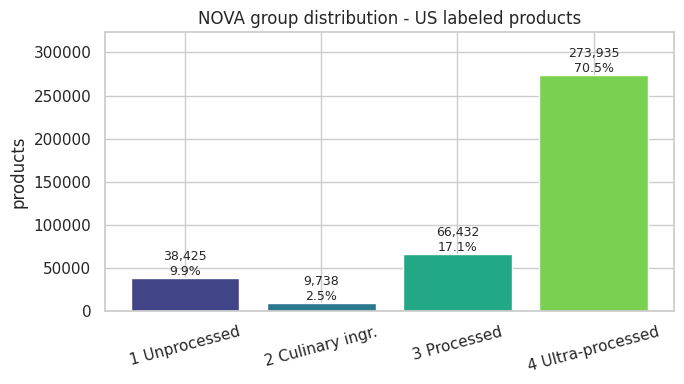
\includegraphics[width=\columnwidth]{class_distribution.png}
\caption{NOVA group distribution of the 388,530 labeled US products.}
\label{fig:classes}
\end{figure}

\subsection{Missing values and the unlabeled population}
Fig.~\ref{fig:missing} compares missing rates for labeled and unlabeled products. Among labeled products, packaging (98\%) and labels (83\%) are almost empty. Core nutrients are missing for 6--21\% and minor nutrients for 23--78\%. Ingredient text, and the ingredient and additive counts derived from it, are missing for only 1.1\% of labeled products but for 88\% of unlabeled ones.

Breaking down the unlabeled products by available inputs makes the consequence clear. Of the 604,627 unlabeled US products:
\begin{itemize}
    \item 69,953 (11.6\%) have ingredient text;
    \item 394,871 (65.3\%) have nutrition facts but neither ingredients nor categories;
    \item 94,718 (15.7\%) have no ingredients, categories or nutrition at all.
\end{itemize}

\begin{figure}[t]
\centering
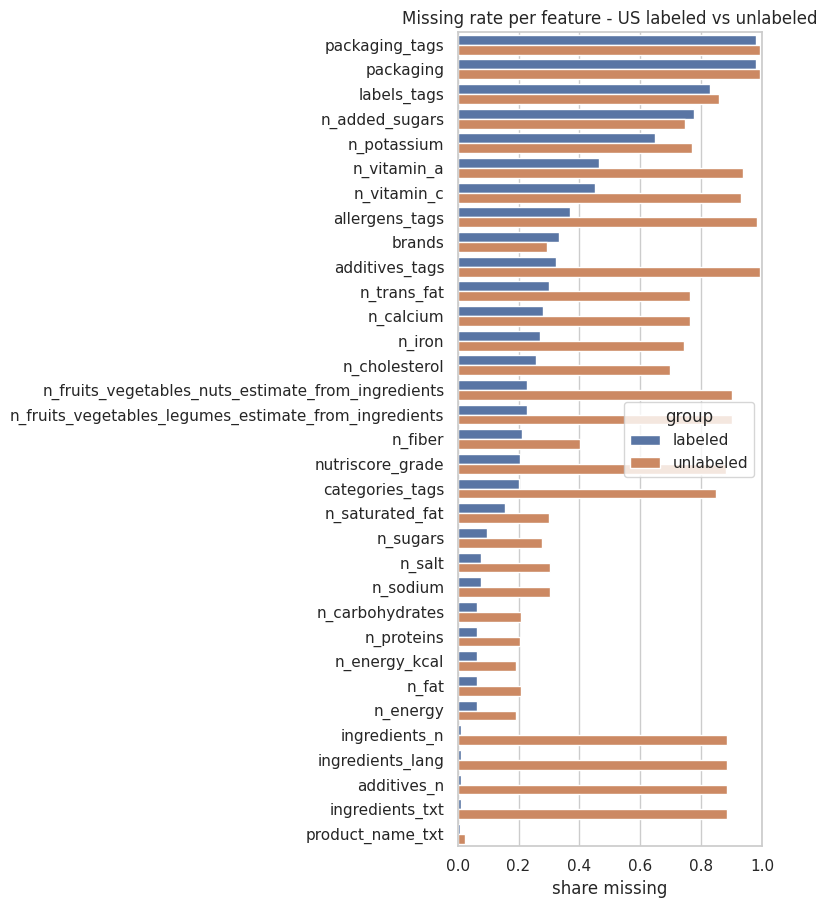
\includegraphics[width=\columnwidth]{missingness.png}
\caption{Missing rate per feature for labeled and unlabeled US products. Ingredient-derived features show the largest gap.}
\label{fig:missing}
\end{figure}

\subsection{Impossible values}
Table~\ref{tab:impossible} lists the most frequent rule violations among labeled products. Raw maxima reach $10^{10}$\,g of sugar per 100\,g, clearly entry errors. After cleaning, every core nutrient lies in $[0, 100]$\,g and energy in $[0, 900]$\,kcal.

\begin{table}[t]
\centering
\caption{Most frequent impossible values (labeled US products)}
\label{tab:impossible}
\begin{tabular}{lrr}
\toprule
Rule violated (per 100\,g) & Products & Share \\
\midrule
Fat + carbohydrates + proteins $>$ 105\,g & 15,441 & 4.0\% \\
Energy $>$ 900\,kcal & 11,277 & 2.9\% \\
Carbohydrates $>$ 100\,g & 10,452 & 2.7\% \\
Sugars $>$ 100\,g & 5,103 & 1.3\% \\
Fat $>$ 100\,g & 4,669 & 1.2\% \\
Proteins $>$ 100\,g & 907 & 0.2\% \\
Sugars $>$ carbohydrates + 0.5\,g & 603 & 0.2\% \\
Saturated fat $>$ fat + 0.5\,g & 410 & 0.1\% \\
\bottomrule
\end{tabular}
\end{table}

\subsection{Nutrients, counts and correlations}
Fig.~\ref{fig:nutrients} shows the core nutrients by NOVA group. NOVA~2 stands apart (median 643\,kcal and 64\,g fat per 100\,g, reflecting oils and fats), while NOVA~3 and~4 have similar fat and energy but differ in sugars and carbohydrates. The ingredient and additive counts separate the classes far more clearly (Fig.~\ref{fig:counts}). NOVA~4 products have a median of 18 ingredients and 3 additives, NOVA~1 products a median of 2 ingredients and none. In the Spearman correlation matrix (Fig.~\ref{fig:corr}), salt and sodium are almost identical ($\rho = 0.995$), since OFF derives one from the other. Saturated fat and fat ($\rho = 0.86$) and fat and energy ($\rho = 0.73$) are also strongly correlated. The additive count ($\rho = 0.65$) and ingredient count ($\rho = 0.61$) correlate far more with NOVA than any nutrient ($|\rho| \le 0.25$).

\begin{figure*}[t]
\centering
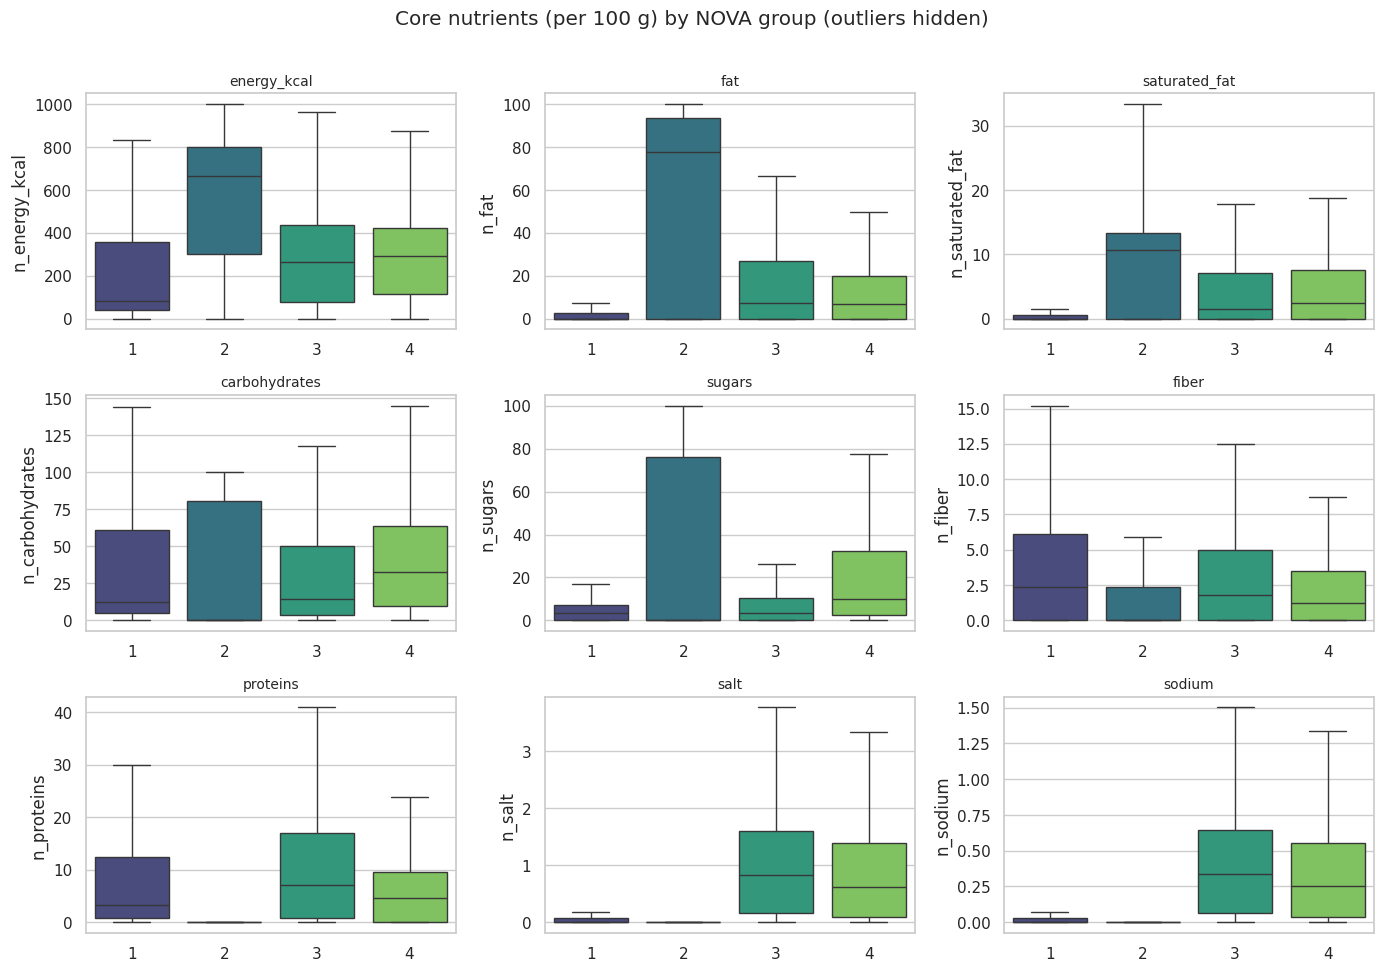
\includegraphics[width=0.8\textwidth]{nutrients_by_nova.png}
\caption{Core nutrients per 100\,g by NOVA group (outliers hidden).}
\label{fig:nutrients}
\end{figure*}

\begin{figure}[t]
\centering
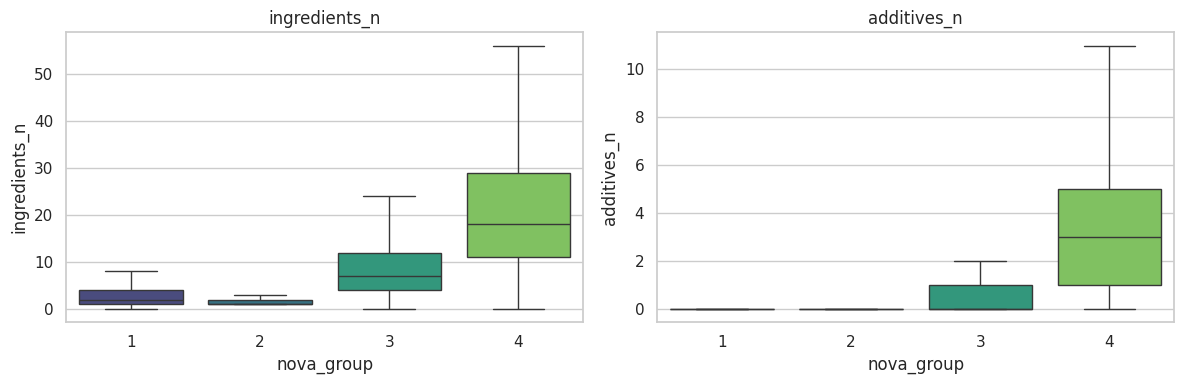
\includegraphics[width=\columnwidth]{counts_by_nova.png}
\caption{Number of ingredients and additives by NOVA group.}
\label{fig:counts}
\end{figure}

\begin{figure}[t]
\centering
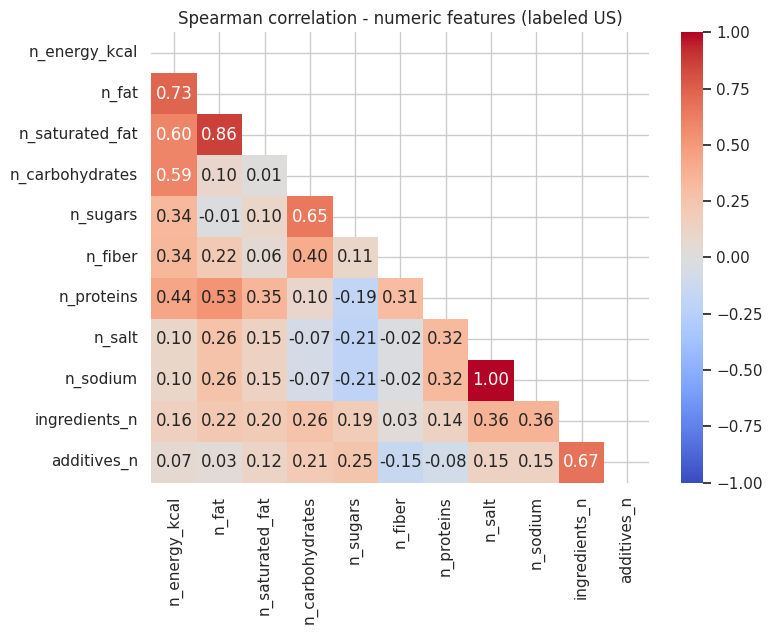
\includegraphics[width=0.92\columnwidth]{spearman_corr.png}
\caption{Spearman correlation among numeric features (labeled US products).}
\label{fig:corr}
\end{figure}

\subsection{Ingredient text and categorical fields}
US ingredient text is almost entirely English: only 0.1\% of texts have more than 5\% non-ASCII characters. It is noisy in other ways:
\begin{itemize}
    \item 14.1\% of texts are mostly upper case;
    \item 2.9\% are shorter than 15 characters;
    \item 18\% duplicate another product's text exactly.
\end{itemize}
Text length grows with processing, from a median of 4 words for NOVA~1 to 36 for NOVA~4 (Fig.~\ref{fig:text}). The most over-represented words per class are interpretable:
\begin{itemize}
    \item NOVA~1: \emph{organic, broccoli, beans};
    \item NOVA~2: \emph{olive, virgin, honey};
    \item NOVA~3: \emph{salt, sea, garlic};
    \item NOVA~4: \emph{natural, flavor, syrup, gum, starch}.
\end{itemize}
Tag fields have high cardinality: 41,629 brands (the top 100 cover only 24\%), 9,844 categories, 2,474 labels, 543 allergens and 515 additives. In addition, 33,585 labeled products carry only the placeholder category \texttt{en:undefined}. Fig.~\ref{fig:categories} shows that some frequent categories are almost pure in NOVA group while others mix all four.

\begin{figure}[t]
\centering
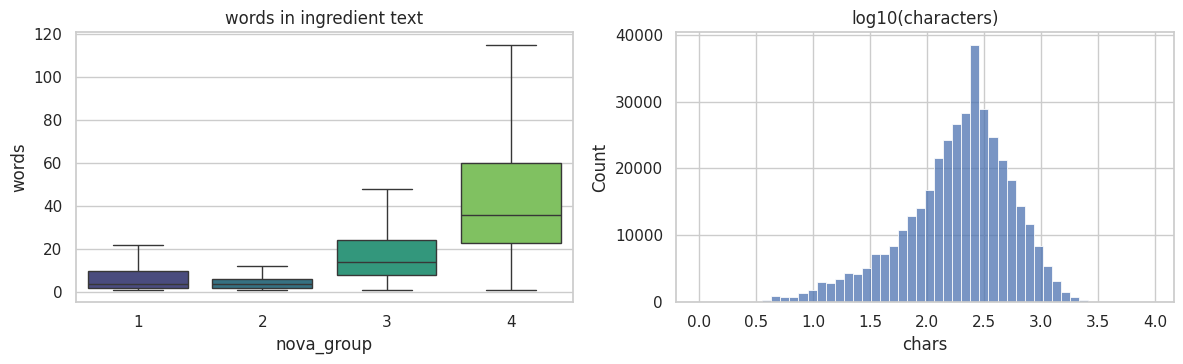
\includegraphics[width=\columnwidth]{text_length.png}
\caption{Words in the ingredient text by NOVA group (left) and distribution of text length (right).}
\label{fig:text}
\end{figure}

\begin{figure}[t]
\centering
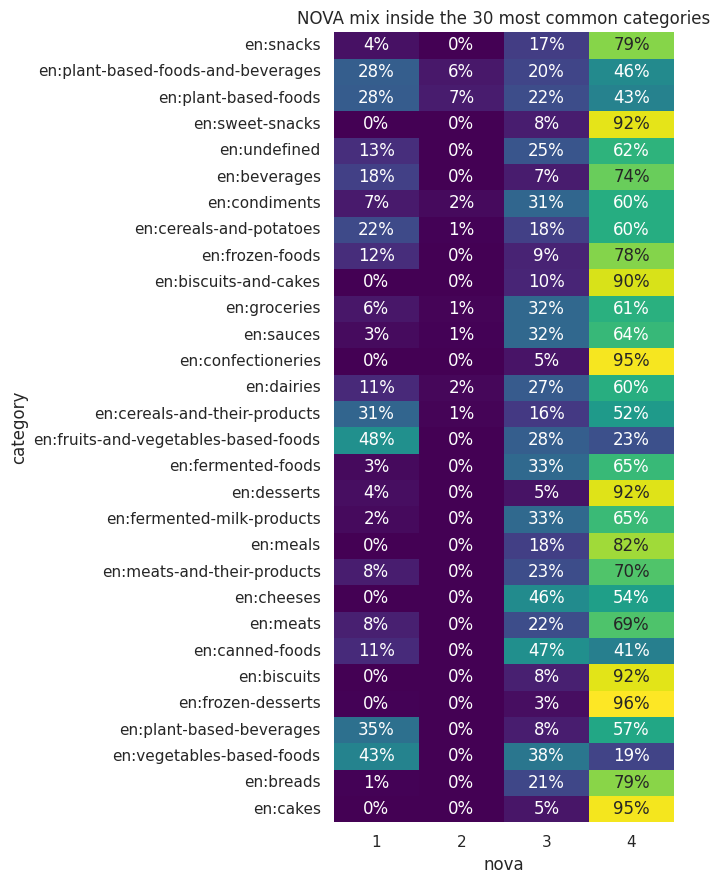
\includegraphics[width=0.85\columnwidth]{category_nova_mix.png}
\caption{Share of each NOVA group inside the 30 most common categories.}
\label{fig:categories}
\end{figure}

\subsection{Sparsity of the text}
TF-IDF on ingredient text (1--2-grams, 60,000-product sample) produces 35,432 features with only 0.17\% non-zero entries. The first 100 SVD components retain just 24.5\% of the variance (Fig.~\ref{fig:svd}).

\begin{figure}[t]
\centering
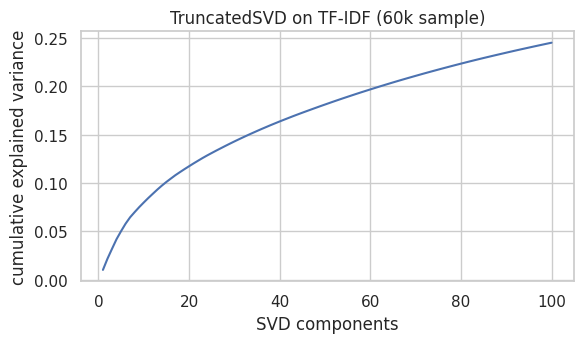
\includegraphics[width=0.85\columnwidth]{svd_variance.png}
\caption{Cumulative explained variance of truncated SVD on TF-IDF ingredient features.}
\label{fig:svd}
\end{figure}

%% =========================================================
\section{Dimensionality Reduction and Clustering}
\label{sec:reduction}

\subsection{The feature space before reduction}
Fig.~\ref{fig:corrall} shows the correlations among all 84 features of the modelling matrix, and Fig.~\ref{fig:pairplot} the four most informative raw features by mutual information on the balanced sample. These are the first text component, the number of words, the ingredient count and the fourth text component. NOVA~4 products extend to longer texts and more ingredients, but all four classes overlap in every pair of features.

\begin{figure}[t]
\centering
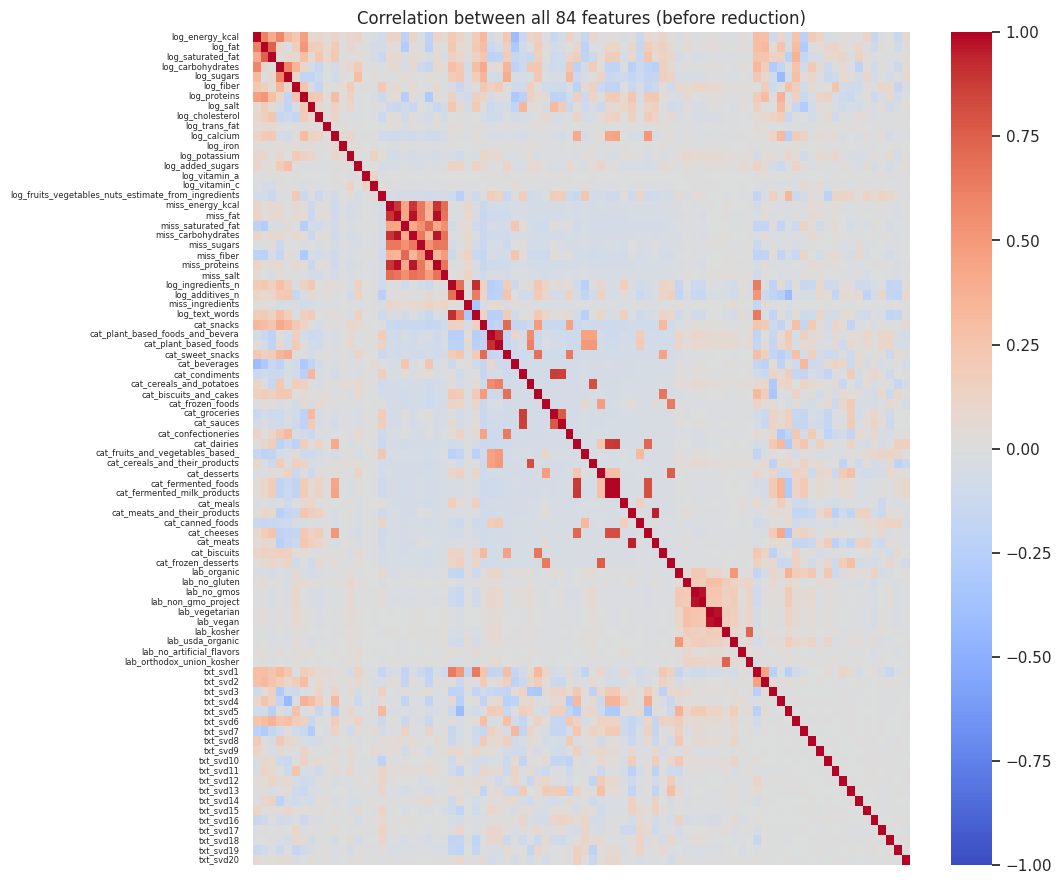
\includegraphics[width=0.95\columnwidth]{corr_all_features.png}
\caption{Correlation between all 84 features before reduction. Blocks of correlated features appear for nutrients, missing flags and related category tags.}
\label{fig:corrall}
\end{figure}

\begin{figure}[t]
\centering
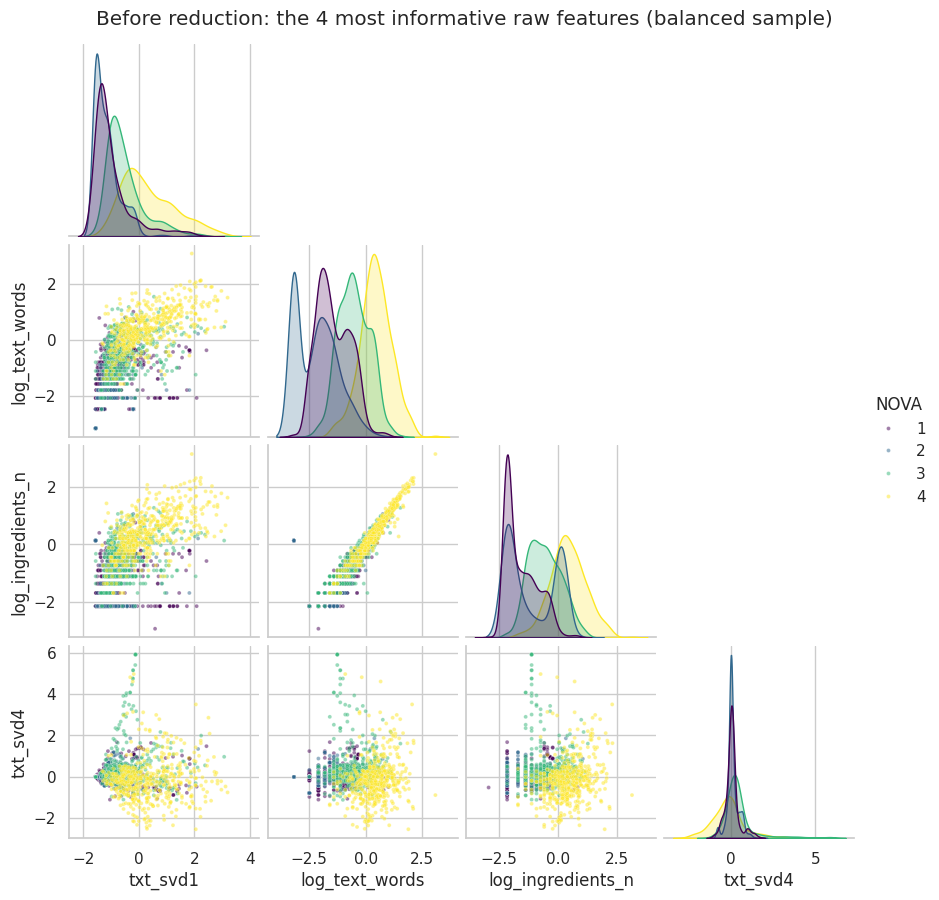
\includegraphics[width=0.9\columnwidth]{pairplot_top4.png}
\caption{The four most informative raw features (mutual information), balanced sample, coloured by NOVA group.}
\label{fig:pairplot}
\end{figure}

\subsection{Linear methods}
PCA needs 46 of the 84 dimensions to keep 90\% of the variance and 56 to keep 95\% (Fig.~\ref{fig:linear}). The information is spread out, with no small set of dominant directions. The first component is a ``product complexity'' axis: its largest loadings are the first text component (0.25), the snack category (0.22), text length (0.22), sweet snacks (0.22), ingredient count (0.22), fat and energy. The second component collects the nutrient missing-value flags (loadings 0.26--0.32): products with an incomplete nutrition panel. LDA's three discriminants carry 60.1\%, 26.3\% and 13.6\% of the between-class variance. The first is driven by the ingredient count, text length, missing ingredient text and the additive count. Truncated SVD gives the same 2-D picture as PCA because the features are already standardised.

\begin{figure*}[t]
\centering
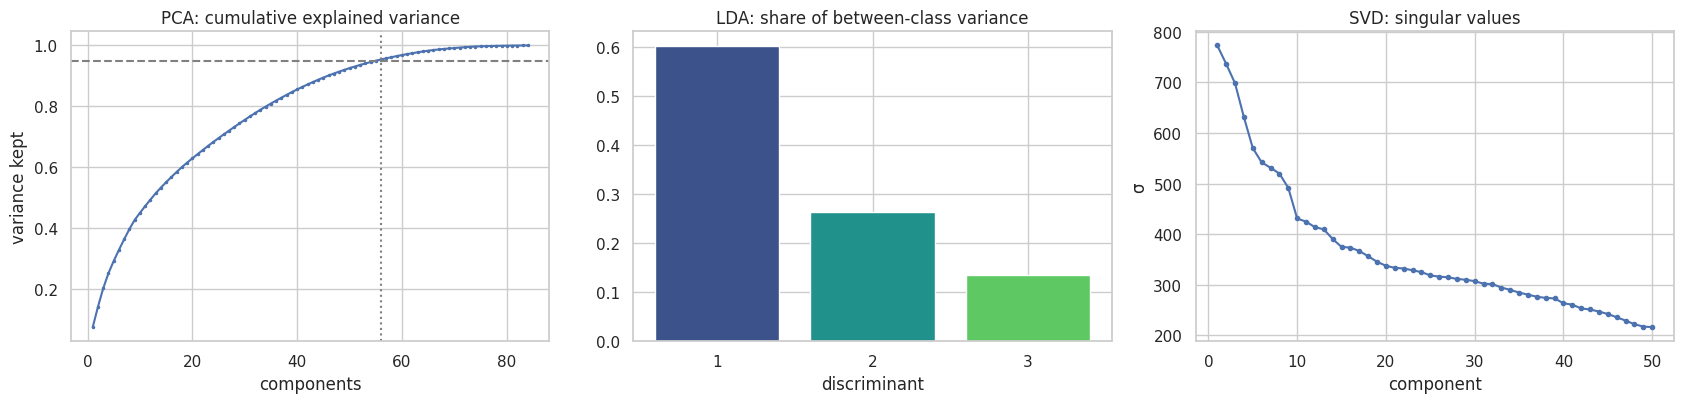
\includegraphics[width=0.9\textwidth]{linear_reduction.png}
\caption{Linear reduction. Left: cumulative variance kept by PCA (95\% at 56 components). Middle: share of between-class variance of the three LDA discriminants. Right: singular values of truncated SVD.}
\label{fig:linear}
\end{figure*}

\subsection{Comparison of all methods}
Fig.~\ref{fig:grid} shows every 2-D embedding coloured by NOVA group, and Table~\ref{tab:dr} scores them.

\begin{figure*}[t]
\centering
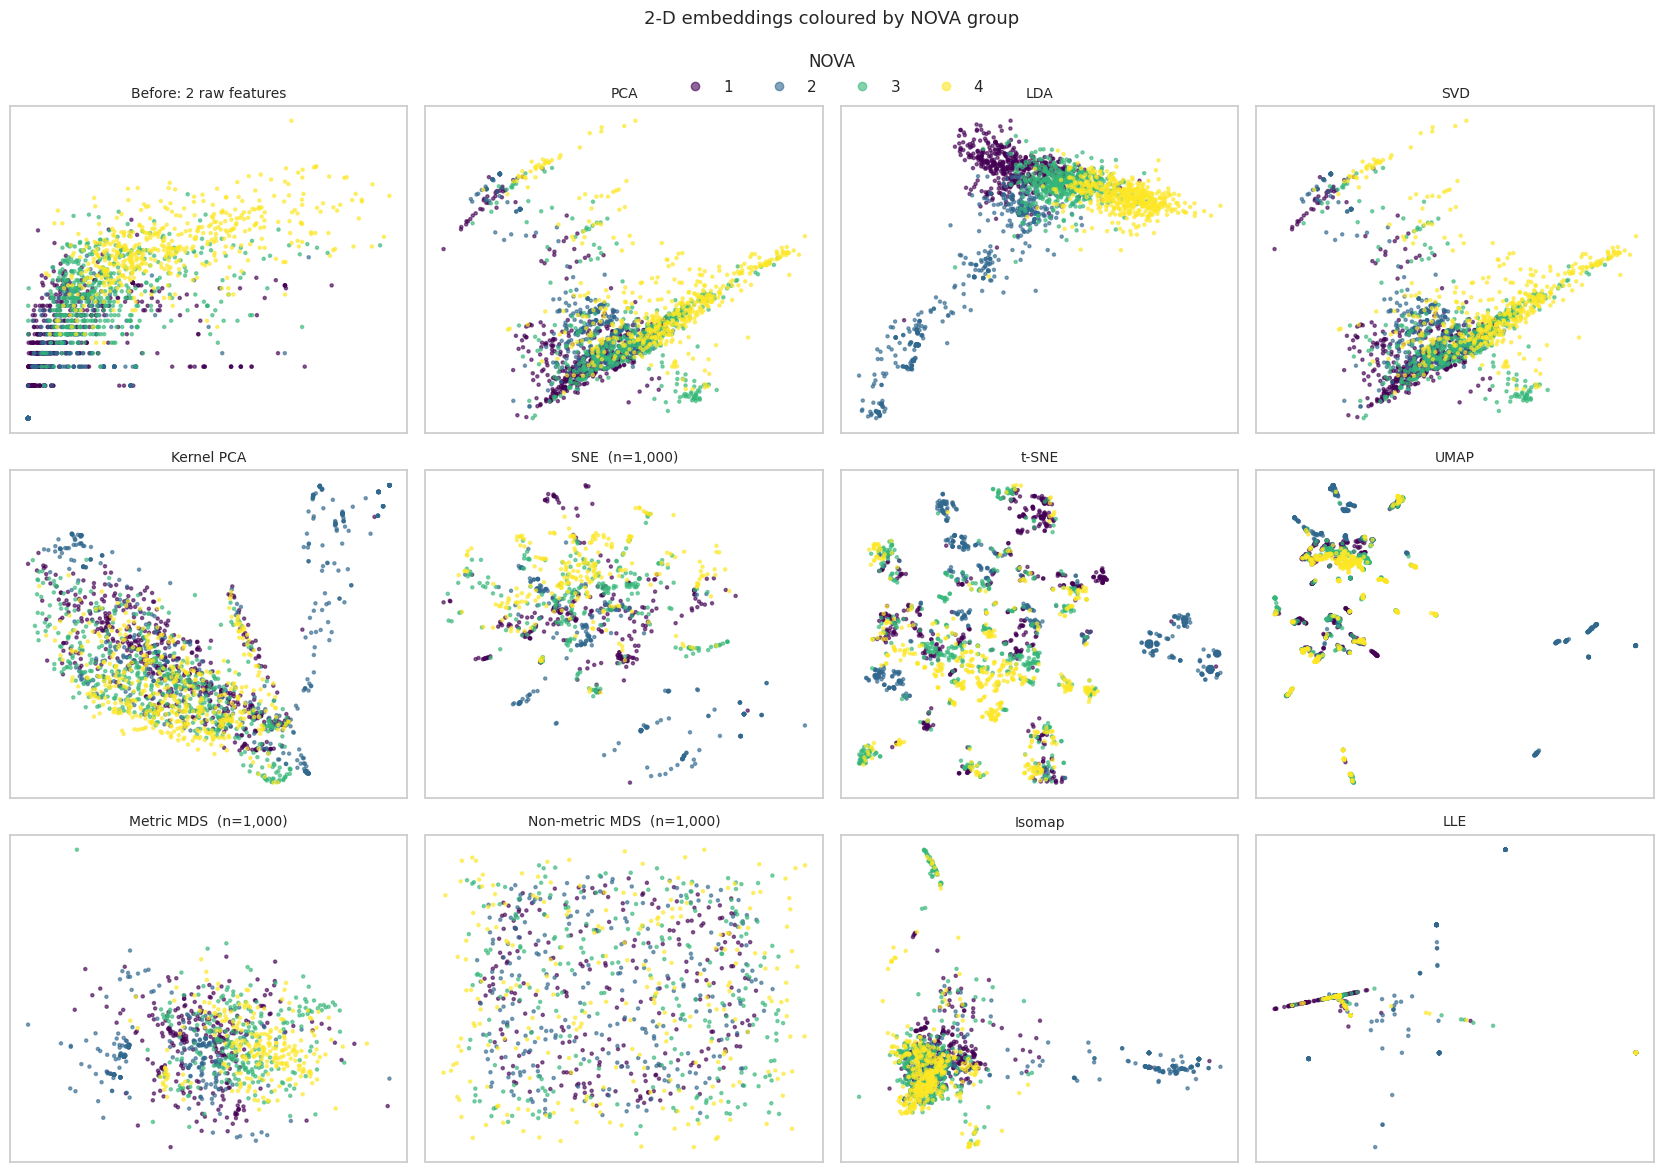
\includegraphics[width=\textwidth]{embeddings_grid.png}
\caption{2-D embeddings of the balanced sample by eleven reduction methods, coloured by NOVA group. The first panel shows the data before reduction (two raw features). MDS and SNE use a 1,000-point subset.}
\label{fig:grid}
\end{figure*}

\begin{table*}[t]
\centering
\caption{Comparison of dimensionality-reduction methods (balanced sample; chance kNN accuracy = 25\%)}
\label{tab:dr}
\setlength{\tabcolsep}{5pt}
\begin{tabular}{lrrrrrrr}
\toprule
Method & Dims & Points & Silhouette (NOVA) & kNN accuracy & Trustworthiness & K-Means ARI & K-Means NMI \\
\midrule
LDA & 2 & 2,000 & \textbf{0.182} & \textbf{79.5\%} & 0.689 & \textbf{0.422} & \textbf{0.491} \\
Original (all features) & 84 & 2,000 & 0.028 & 77.3\% & 1.000 & 0.054 & 0.207 \\
t-SNE & 2 & 2,000 & $-0.032$ & 73.5\% & \textbf{0.983} & 0.067 & 0.089 \\
UMAP & 2 & 2,000 & $-0.055$ & 71.7\% & 0.976 & 0.056 & 0.147 \\
SNE (ours) & 2 & 1,000 & $-0.026$ & 68.0\% & 0.905 & 0.109 & 0.165 \\
Metric MDS & 2 & 1,000 & $-0.006$ & 61.5\% & 0.814 & 0.101 & 0.128 \\
PCA & 2 & 2,000 & $-0.006$ & 58.4\% & 0.757 & 0.104 & 0.146 \\
SVD & 2 & 2,000 & $-0.006$ & 58.4\% & 0.757 & 0.104 & 0.146 \\
LLE & 2 & 2,000 & $-0.206$ & 52.4\% & 0.769 & 0.018 & 0.123 \\
Kernel PCA (RBF) & 2 & 2,000 & $-0.062$ & 51.3\% & 0.727 & 0.044 & 0.102 \\
Isomap & 2 & 2,000 & $-0.106$ & 49.5\% & 0.765 & 0.056 & 0.162 \\
Non-metric MDS$^\dagger$ & 2 & 1,000 & $-0.051$ & 34.9\% & 0.510 & 0.000 & 0.003 \\
\bottomrule
\multicolumn{8}{l}{\footnotesize $^\dagger$Did not converge: the solver stopped after its first iteration and returned its random initial layout (0.5\,s).}
\end{tabular}
\end{table*}

Three groups emerge. \textbf{LDA}, the only supervised method, is the only one in which the classes form separate regions. It even beats the full 84-dimensional space on kNN accuracy (79.5\% vs 77.3\%), because it compresses exactly the directions that separate the classes. \textbf{Neighbourhood methods} (t-SNE, UMAP, SNE) preserve local structure best: t-SNE keeps 98\% trustworthiness and 73.5\% kNN accuracy in two dimensions. They produce many small, tight islands of products, many of them dominated by one or two NOVA groups. \textbf{Global methods} (PCA, SVD, metric MDS, Kernel PCA, Isomap, LLE) preserve distances or variance over the whole sample and lose more than half of the class information in two dimensions. LLE and Isomap collapse most points into a dense core with a few long arms of NOVA~2 products (oils, sugars), which are the most distinct group.

Our SNE implementation converged: the KL cost fell from about 3,500 to 1,650 and levelled off after about 150 iterations. It reaches 68.0\% kNN accuracy, below t-SNE, as expected from the crowding problem that t-SNE was designed to fix: points of different islands are pushed together in the centre of the SNE map. Non-metric MDS failed to converge in our run, and its row should be read as a failed run rather than a property of the data. Initialising it from the metric MDS solution would fix this.

\subsection{Clustering before and after reduction}
K-Means with four clusters does not rediscover the NOVA groups in the original 84-dimensional space (ARI 0.054, NMI 0.207). The elbow and silhouette curves (Fig.~\ref{fig:elbow}) show no natural cut at $k=4$. The cluster silhouette peaks at $k=3$ and drops sharply at $k=4$. Fig.~\ref{fig:clusters} compares true groups and clusters before and after reduction. In t-SNE and UMAP space the clusters group the many small islands of similar products together, and these groups cut across processing levels (ARI 0.06--0.07). Only in LDA space, which already uses the labels, do the clusters agree with NOVA (ARI 0.422). There one cluster captures the elongated arm of NOVA~2 and the others divide the band from NOVA~1 to NOVA~4.

\begin{figure}[t]
\centering
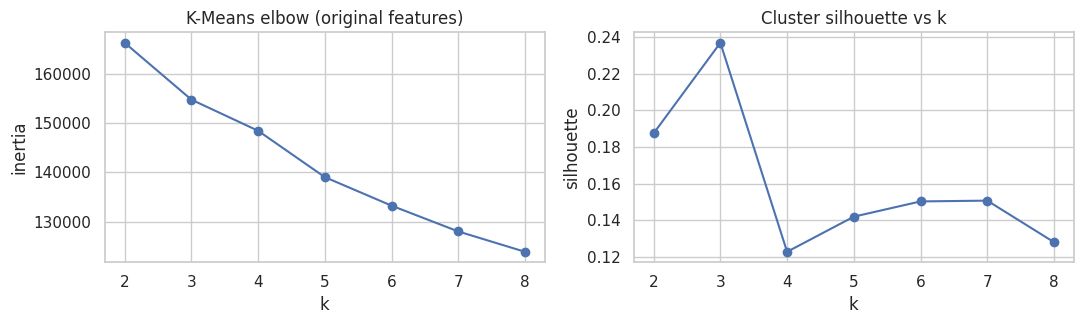
\includegraphics[width=\columnwidth]{kmeans_elbow.png}
\caption{K-Means on the original features: inertia (elbow) and cluster silhouette for $k = 2,\dots,8$.}
\label{fig:elbow}
\end{figure}

\begin{figure*}[t]
\centering
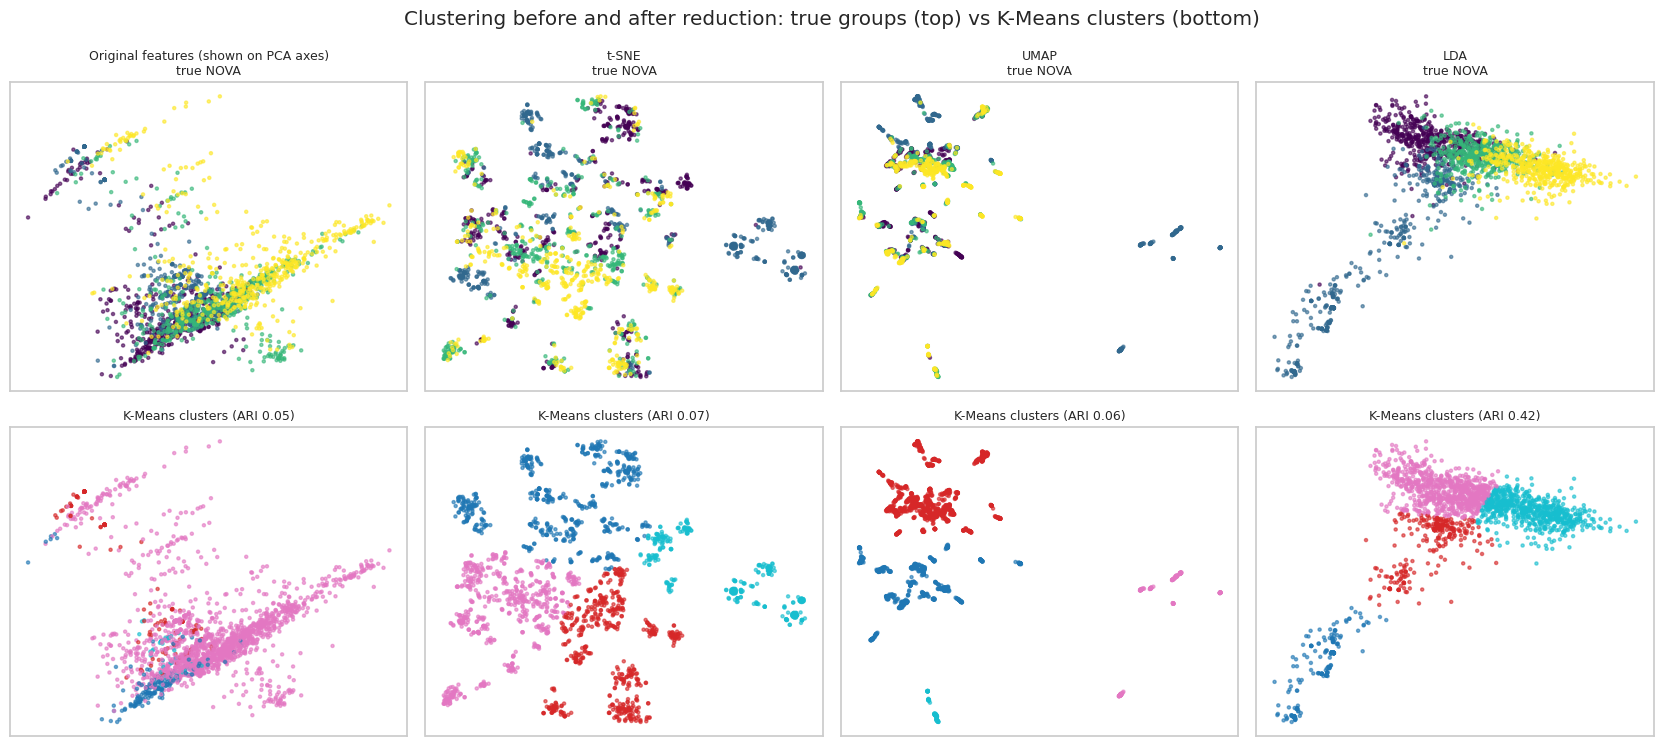
\includegraphics[width=0.95\textwidth]{clustering_before_after.png}
\caption{Clustering before and after reduction. Top: true NOVA groups. Bottom: K-Means clusters ($k=4$) with their ARI against NOVA. From left: original features (shown on PCA axes), t-SNE, UMAP, LDA.}
\label{fig:clusters}
\end{figure*}

%% =========================================================
\section{Feature Selection}
\label{sec:selection}

With all 84 features the common evaluator reaches a cross-validated macro-F1 of 0.874. Table~\ref{tab:fs} compares all twelve methods.

\begin{table}[t]
\centering
\caption{Feature-selection methods scored by the same evaluator (3-fold CV macro-F1, gradient boosting, 20,000 training products)}
\label{tab:fs}
\begin{tabular}{llrrr}
\toprule
Method & Family & Feat. & Macro-F1 & $\Delta$ \\
\midrule
None (all features) & -- & 84 & 0.874 & -- \\
Elastic Net & Embedded & 82 & 0.873 & $-0.001$ \\
L1 (Lasso) & Embedded & 78 & 0.870 & $-0.004$ \\
Correlation ($|r|\le0.9$) & Filter & 76 & 0.866 & $-0.008$ \\
Binary PSO & Metaheur. & 51 & 0.865 & $-0.009$ \\
Genetic algorithm & Metaheur. & 45 & 0.861 & $-0.013$ \\
Forward selection & Wrapper & 15 & 0.843 & $-0.031$ \\
ANOVA $F$ (top 20) & Filter & 20 & 0.842 & $-0.033$ \\
L2 (Ridge, top 20) & Embedded & 20 & 0.836 & $-0.038$ \\
Mutual inf. (top 20) & Filter & 20 & 0.835 & $-0.040$ \\
Backward elimination & Wrapper & 15 & 0.834 & $-0.040$ \\
RFE & Wrapper & 15 & 0.832 & $-0.042$ \\
$\chi^2$ (top 20) & Filter & 20 & 0.747 & $-0.127$ \\
\bottomrule
\end{tabular}
\end{table}

\subsection{Filter methods}
Sixteen features are nearly constant after min-max scaling. They are mostly minor nutrients (cholesterol, trans fat, calcium, iron, potassium, vitamins A and C, which are tiny per 100\,g) and some weak text components. The three ranking filters disagree in instructive ways (Fig.~\ref{fig:filter}). Mutual information favours the text components, text length and the two counts. ANOVA $F$ favours text length and the counts first, then categories and nutrients. $\chi^2$ is dominated by sparse binary indicators: missing ingredient text, plant-based and fruit-and-vegetable categories, and the organic label. Its subset scores far lower (0.747) because a rare indicator can have a large $\chi^2$ while helping few products. The correlation filter removes only 8 features, which confirms that most features are not linearly redundant.

\begin{figure*}[t]
\centering
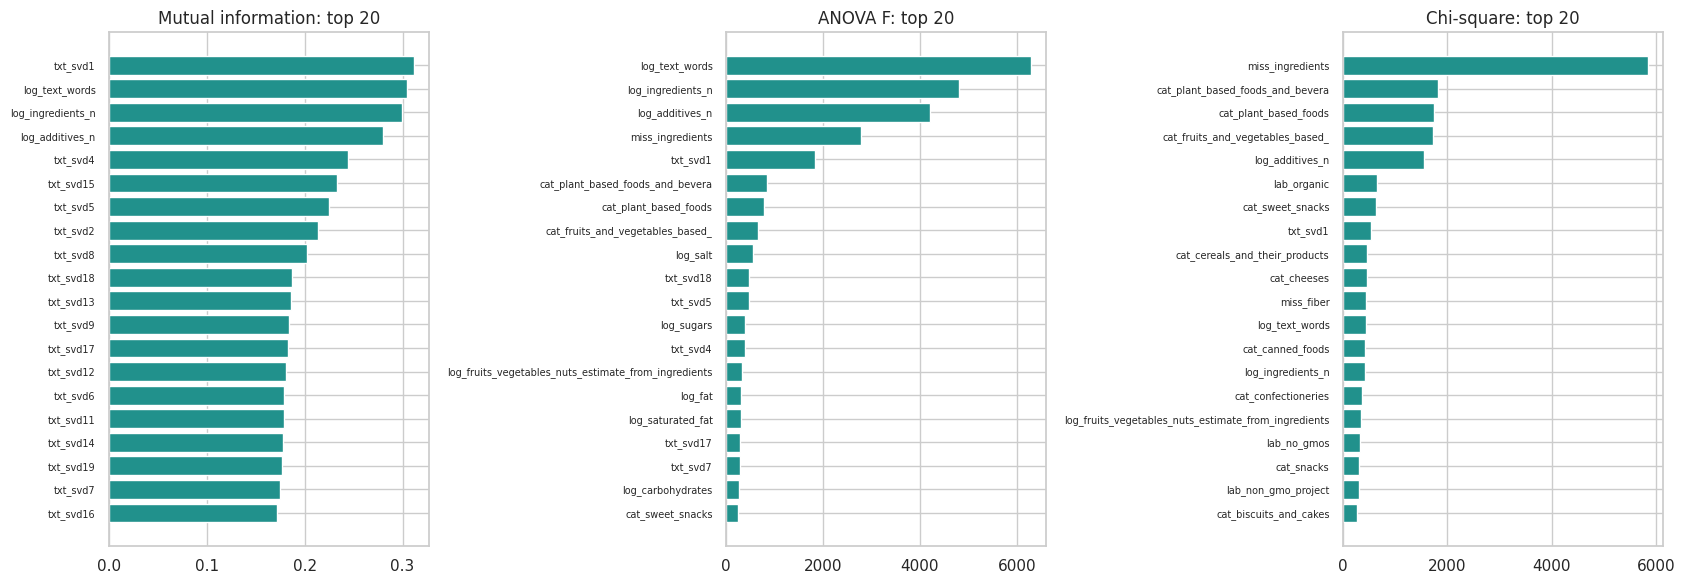
\includegraphics[width=0.95\textwidth]{filter_scores.png}
\caption{Filter methods: top 20 features by mutual information, ANOVA $F$ and $\chi^2$ (training sample).}
\label{fig:filter}
\end{figure*}

\subsection{Wrapper methods}
Forward selection took 36\,s, backward elimination 96\,s and RFE 42\,s. All three converge on a similar core: the additive count, text length, a set of text components, and three or four nutrients (salt, fat, proteins, sugars or carbohydrates). Forward selection scored best of the 15-feature subsets (0.843). RFE, which searches all 84 features, also picks the snack, sweet-snack and beverage categories.

\subsection{Embedded methods}
With $C=0.05$, the L1 penalty removes only 6 features, and Elastic Net only 2 (Fig.~\ref{fig:embedded}). Most features carry some independent information for at least one class. The coefficients are also interpretable. The additive count, the first text component and the ingredient count push strongly towards NOVA~4. Text component~7 pushes towards NOVA~1. Missing ingredient text pushes towards NOVA~2, and the beverage and snack categories push strongly away from it. Elastic Net keeps 82 features with essentially no loss and was therefore chosen as the ``selected'' feature set for the classifiers, although the gain over all 84 features is negligible.

\begin{figure*}[t]
\centering
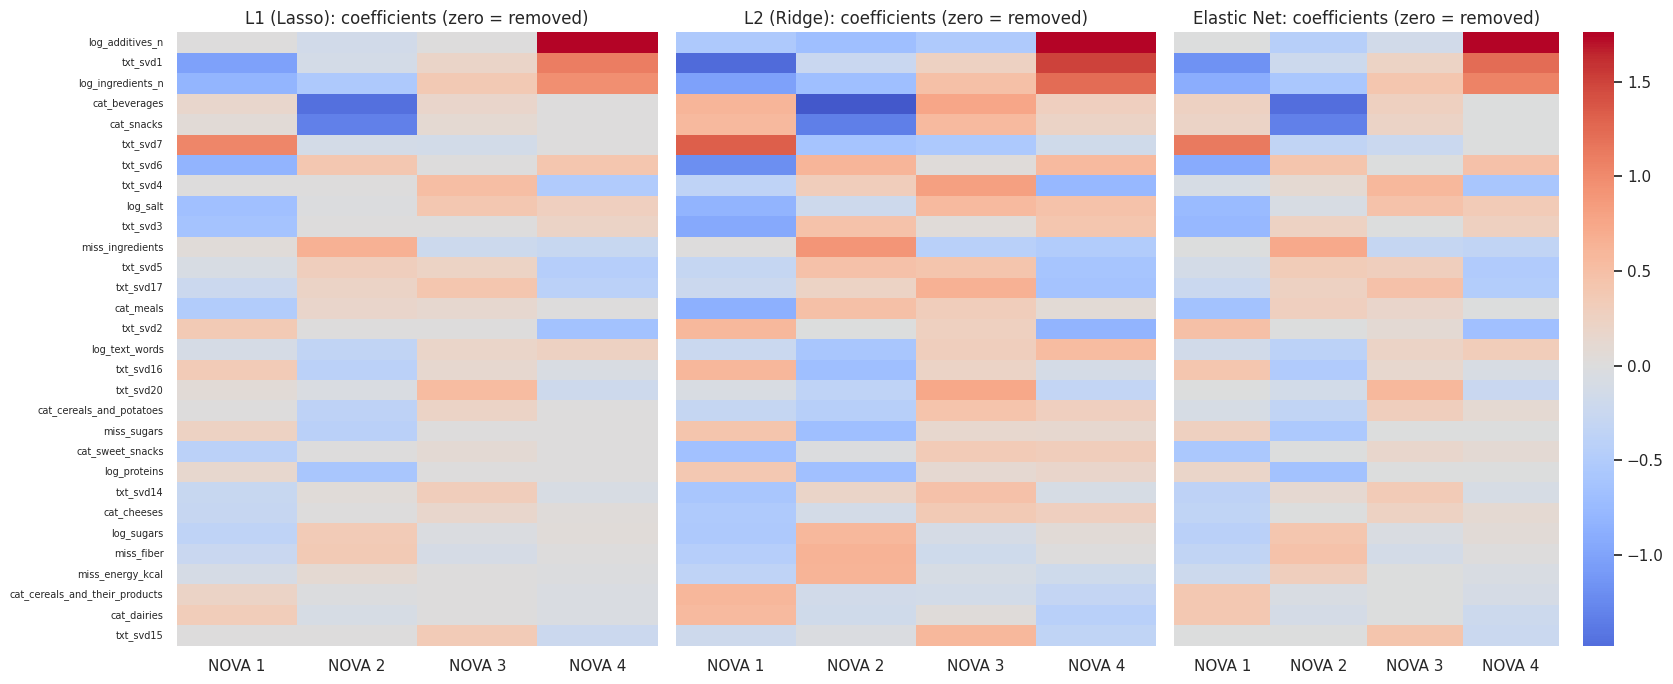
\includegraphics[width=0.95\textwidth]{embedded_coefficients.png}
\caption{Embedded methods: logistic-regression coefficients per class under L1, L2 and Elastic Net penalties for the 30 most important features (zero = removed).}
\label{fig:embedded}
\end{figure*}

\subsection{Metaheuristics}
Both searches improved steadily (Fig.~\ref{fig:gapso}). The genetic algorithm raised its best fitness from 0.747 to 0.805 over 20 generations (423 distinct subsets evaluated, 223\,s), with the population mean following closely behind. Binary PSO reached 0.794 after 15 iterations (153\,s), with a noisier swarm mean, typical of the stochastic bit sampling. The metaheuristics found the best trade-off between size and score. The GA keeps 54\% of the features (45) and loses only 1.5\% of the score, and PSO keeps 51 features and loses 1.0\%.

\begin{figure}[t]
\centering
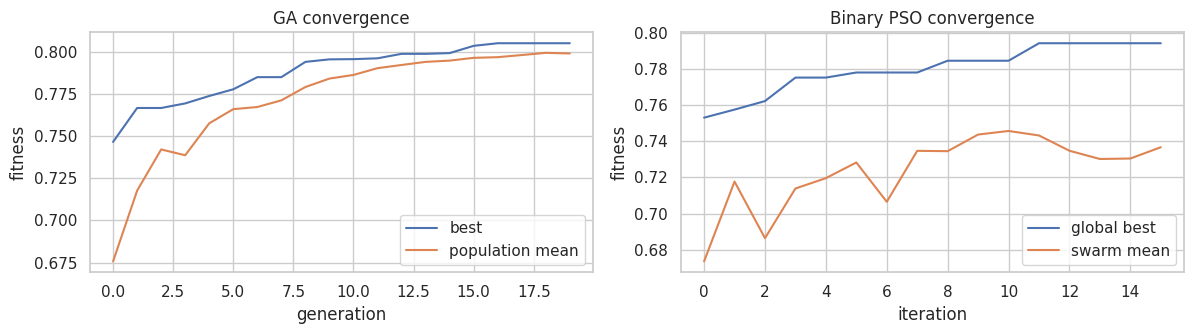
\includegraphics[width=\columnwidth]{ga_pso_convergence.png}
\caption{Convergence of the genetic algorithm (left) and binary PSO (right): best and mean fitness per generation or iteration.}
\label{fig:gapso}
\end{figure}

Across all twelve methods, the features chosen most often are the additive count (selected by nearly every method), the first text components, text length, salt, the ingredient count, missing ingredient text, and the snack categories. These form the core signal of the dataset.

%% =========================================================
\section{Classification Results}
\label{sec:models}

\subsection{Test-set performance}
Table~\ref{tab:models} reports all fifteen model--feature-set combinations on the 24,000-product test set, and Fig.~\ref{fig:modelbars} compares their macro-F1. The tree ensembles lead on every feature set. The best model is the Random Forest on all features: 93.8\% accuracy (error rate 6.2\%), macro-F1 0.910, weighted F1 0.937 and ROC-AUC 0.990. Gradient boosting follows closely (macro-F1 0.896). It has the highest macro recall (0.925) but lower precision (0.872), i.e.\ it predicts the small classes more often. Logistic regression has high recall (0.883) but the lowest precision (0.751): its linear boundaries, combined with class weights, over-predict NOVA~2 and NOVA~3.

Feature selection changes macro-F1 by at most 0.004. PCA costs the tree models the most (Decision Tree $-0.086$, Random Forest $-0.041$), because rotating the features destroys the axis-aligned splits that trees exploit. kNN, which only uses distances, is unchanged (0.829 vs 0.826).

\begin{table*}[t]
\centering
\caption{Test-set results (24,000 products) for five classifiers on three feature sets, sorted by macro-F1}
\label{tab:models}
\setlength{\tabcolsep}{4.5pt}
\begin{tabular}{llrrrrrrrrr}
\toprule
Features & Model & Feat. & Accuracy & Error & Prec. (macro) & Recall (macro) & F1 (macro) & F1 (weighted) & ROC-AUC & Fit (s) \\
\midrule
All & Random Forest & 84 & \textbf{0.938} & \textbf{0.062} & \textbf{0.917} & 0.904 & \textbf{0.910} & \textbf{0.937} & \textbf{0.990} & 86 \\
Selected & Random Forest & 82 & 0.937 & 0.063 & 0.915 & 0.904 & 0.909 & 0.937 & 0.990 & 88 \\
All & Gradient Boosting & 84 & 0.920 & 0.080 & 0.872 & \textbf{0.925} & 0.896 & 0.923 & 0.989 & 23 \\
Selected & Gradient Boosting & 82 & 0.918 & 0.082 & 0.866 & 0.923 & 0.892 & 0.921 & 0.989 & 22 \\
PCA & Random Forest & 56 & 0.909 & 0.091 & 0.894 & 0.849 & 0.869 & 0.906 & 0.981 & 201 \\
All & Decision Tree & 84 & 0.899 & 0.101 & 0.861 & 0.862 & 0.862 & 0.899 & 0.904 & 8 \\
Selected & Decision Tree & 82 & 0.899 & 0.101 & 0.858 & 0.862 & 0.860 & 0.899 & 0.905 & 9 \\
PCA & Gradient Boosting & 56 & 0.887 & 0.113 & 0.827 & 0.894 & 0.856 & 0.892 & 0.981 & 17 \\
PCA & kNN ($k$=15) & 56 & 0.884 & 0.116 & 0.840 & 0.821 & 0.829 & 0.881 & 0.966 & 0 \\
Selected & kNN ($k$=15) & 82 & 0.882 & 0.118 & 0.835 & 0.821 & 0.827 & 0.879 & 0.966 & 0 \\
All & kNN ($k$=15) & 84 & 0.882 & 0.118 & 0.836 & 0.820 & 0.826 & 0.879 & 0.965 & 0 \\
All & Logistic Regression & 84 & 0.866 & 0.134 & 0.751 & 0.883 & 0.804 & 0.873 & 0.976 & 10 \\
Selected & Logistic Regression & 82 & 0.866 & 0.134 & 0.751 & 0.883 & 0.804 & 0.873 & 0.976 & 11 \\
PCA & Logistic Regression & 56 & 0.855 & 0.145 & 0.733 & 0.870 & 0.788 & 0.862 & 0.971 & 9 \\
PCA & Decision Tree & 56 & 0.844 & 0.156 & 0.773 & 0.779 & 0.776 & 0.844 & 0.849 & 20 \\
\bottomrule
\end{tabular}
\end{table*}

\begin{figure}[t]
\centering
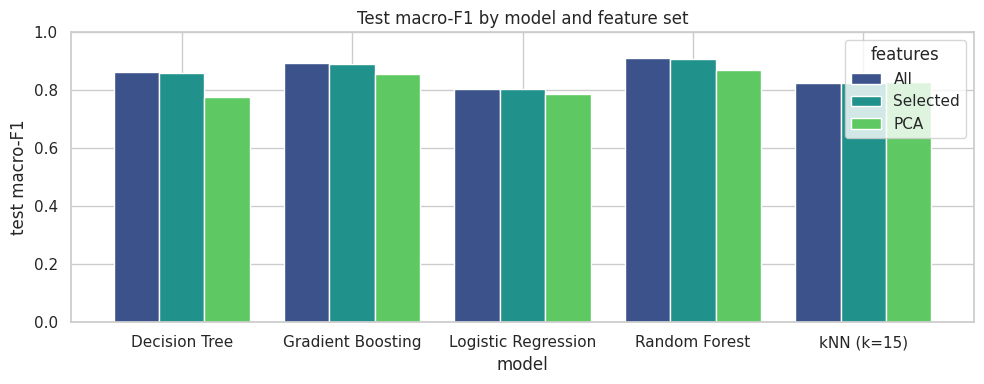
\includegraphics[width=\columnwidth]{model_f1_bars.png}
\caption{Test macro-F1 by model and feature set.}
\label{fig:modelbars}
\end{figure}

\subsection{Per-class results and confusion matrices}
Table~\ref{tab:perclass} gives the per-class results of the best model, and Fig.~\ref{fig:cmall} the row-normalised confusion matrices of all five models on all features. Fig.~\ref{fig:bestcm} shows the best model's confusion matrix in counts, with its one-vs-rest ROC curves. Per-class AUC is 0.996 for NOVA~1, 0.998 for NOVA~2, 0.979 for NOVA~3 and 0.988 for NOVA~4.

\begin{table}[t]
\centering
\caption{Per-class results of the best model (Random Forest, all features)}
\label{tab:perclass}
\begin{tabular}{lrrrr}
\toprule
Class & Precision & Recall & F1 & Support \\
\midrule
1 Unprocessed & 0.924 & 0.933 & 0.929 & 2,374 \\
2 Culinary ingredients & 0.922 & 0.909 & 0.915 & 601 \\
3 Processed & 0.865 & 0.803 & 0.833 & 4,104 \\
4 Ultra-processed & 0.956 & 0.972 & 0.964 & 16,921 \\
\midrule
Macro average & 0.917 & 0.904 & 0.910 & 24,000 \\
Weighted average & 0.937 & 0.938 & 0.937 & 24,000 \\
\bottomrule
\end{tabular}
\end{table}

\begin{figure*}[t]
\centering
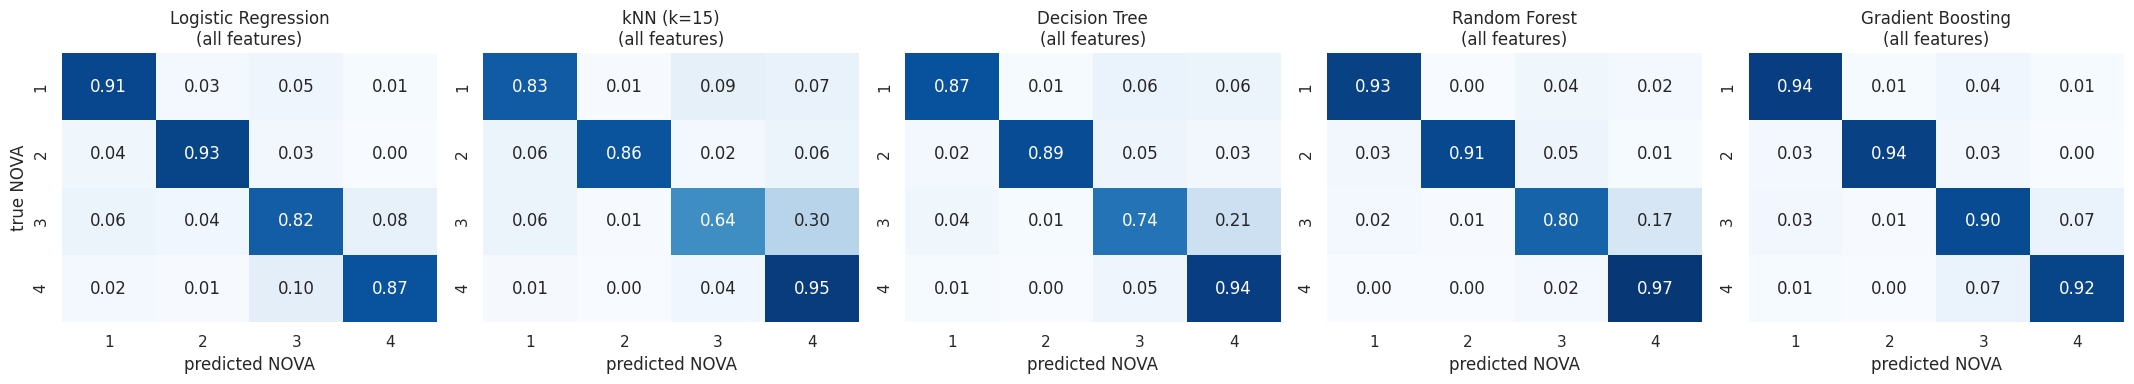
\includegraphics[width=\textwidth]{confusion_all_models.png}
\caption{Row-normalised confusion matrices of the five classifiers on all features (diagonal = per-class recall).}
\label{fig:cmall}
\end{figure*}

\begin{figure*}[t]
\centering
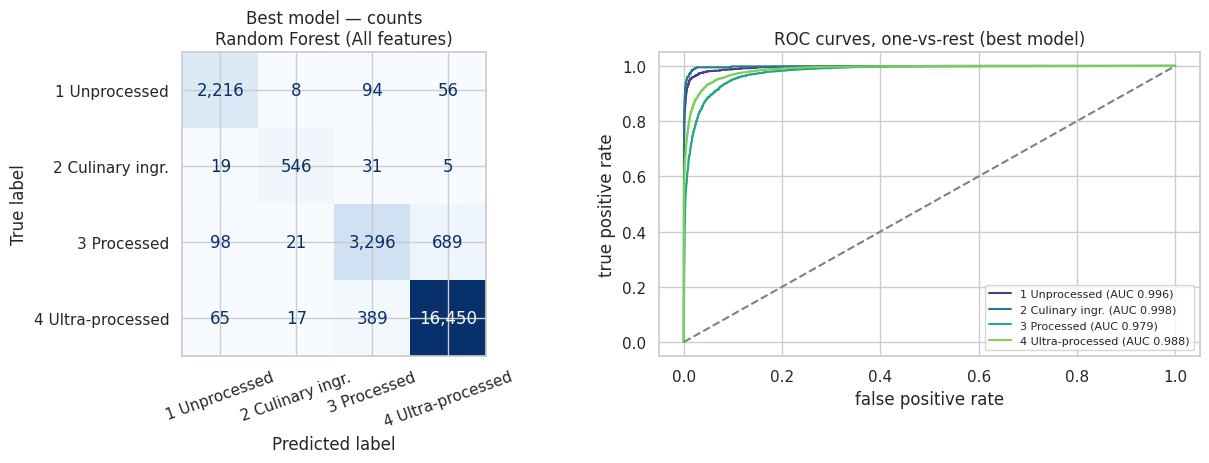
\includegraphics[width=0.85\textwidth]{best_cm_roc.png}
\caption{Best model (Random Forest, all features). Left: confusion matrix in counts. Right: one-vs-rest ROC curves with per-class AUC.}
\label{fig:bestcm}
\end{figure*}

\textbf{Interpreting the confusion matrix.}
\begin{itemize}
    \item \textbf{Per-class recall.} The best model recognises ultra-processed foods best (recall 97.2\%) and processed foods worst (80.3\%). Unprocessed foods and culinary ingredients are recognised well (93.3\% and 90.8\%) despite being 10\% and 2.5\% of the data, which shows that class weighting and the distinctive profiles of these groups compensate for their size.
    \item \textbf{Largest error.} The largest single error is 689 processed products (16.8\% of NOVA~3) predicted as ultra-processed. In the other direction, 389 ultra-processed products are predicted as processed. NOVA~3 and NOVA~4 differ mainly in the presence of a few marker ingredients or additives, which may be listed under many names, or not at all in a short crowd-entered text.
    \item \textbf{Neighbouring groups.} 78\% of all errors are between neighbouring groups (1$\leftrightarrow$2, 2$\leftrightarrow$3, 3$\leftrightarrow$4). The model usually misjudges the degree of processing by one step rather than confusing opposite ends. Only 56 unprocessed products are labeled ultra-processed, and 65 the other way.
    \item \textbf{Direction of errors.} More errors push products towards a more processed group (883) than a less processed one (609). For a consumer-facing warning this is the safer direction.
\end{itemize}
The other models show the same structure with more errors. Logistic regression mainly loses precision by predicting NOVA~3 for 10\% of NOVA~4 products.

\subsection{Cross-validation and fit diagnosis}
Table~\ref{tab:cv} reports 5-fold cross-validation and the fit diagnosis. Fold-to-fold standard deviations are small (at most 0.008 macro-F1), so the ranking of models is stable. Cross-validation uses 30,000 training products, so its scores are lower than the test scores of models trained on 96,000. The Random Forest drops from 0.910 to 0.880 and gradient boosting from 0.896 to 0.878. This already shows that the models benefit from more data.

\begin{table*}[t]
\centering
\caption{5-fold cross-validation (30,000 training products) and over/underfitting diagnosis (all features)}
\label{tab:cv}
\setlength{\tabcolsep}{5pt}
\begin{tabular}{lrrrrrl}
\toprule
Model & CV accuracy & CV macro-F1 & Train macro-F1 & Test macro-F1 & Gap & Diagnosis \\
\midrule
Logistic Regression & 0.869 $\pm$ 0.003 & 0.815 $\pm$ 0.004 & 0.820 & 0.804 & 0.015 & Good fit \\
kNN ($k$=15) & 0.855 $\pm$ 0.004 & 0.785 $\pm$ 0.006 & 0.851 & 0.826 & 0.025 & Good fit \\
Decision Tree & 0.870 $\pm$ 0.004 & 0.809 $\pm$ 0.008 & 0.999 & 0.862 & 0.138 & Overfitting \\
Random Forest & \textbf{0.919} $\pm$ 0.002 & \textbf{0.880} $\pm$ 0.006 & 0.991 & \textbf{0.910} & 0.081 & Overfitting \\
Gradient Boosting & 0.908 $\pm$ 0.001 & 0.878 $\pm$ 0.004 & 0.934 & 0.896 & 0.039 & Good fit \\
\bottomrule
\end{tabular}
\end{table*}

\begin{figure*}[t]
\centering
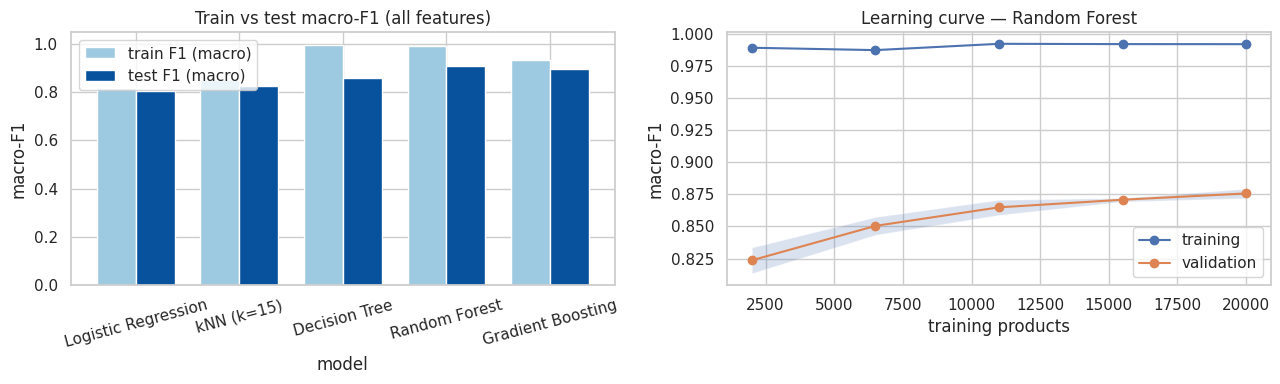
\includegraphics[width=0.85\textwidth]{fit_learning_curve.png}
\caption{Left: training vs test macro-F1 for each model (all features). Right: learning curve of the Random Forest (3-fold CV on up to 20,000 products).}
\label{fig:fit}
\end{figure*}

The fully grown decision tree memorises the training set (training macro-F1 0.999, test 0.862): classic overfitting. The Random Forest also has a training score near 1 (0.991) and a gap of 0.081, just above our threshold, but it has the best test score of all models. Its learning curve (Fig.~\ref{fig:fit}) shows why this overfitting is benign. The validation score keeps rising, from 0.82 at 2,000 products to 0.88 at 20,000, while the training score stays near 0.99. More data, not less model complexity, is the lever. Gradient boosting has the smallest gap of the strong models (0.039). Logistic regression and kNN fit well but are limited by their simpler decision boundaries. No model underfits: all test macro-F1 scores exceed 0.80.

\subsection{Ablation by feature group}
\label{sec:ablation}
Table~\ref{tab:ablation} retrains gradient boosting on single feature groups.

\begin{table}[t]
\centering
\caption{Ablation by feature group (gradient boosting, test set)}
\label{tab:ablation}
\begin{tabular}{lrrrr}
\toprule
Features & Count & Acc. & F1 (mac.) & AUC \\
\midrule
All features & 84 & 0.920 & 0.896 & 0.989 \\
Without ingr./additive counts & 82 & 0.897 & 0.872 & 0.985 \\
Ingredient text only & 24 & 0.904 & 0.846 & 0.983 \\
Nutrients only (+ flags) & 25 & 0.750 & 0.696 & 0.923 \\
Categories + labels only & 35 & 0.445 & 0.391 & 0.794 \\
\bottomrule
\end{tabular}
\end{table}

The ingredient text, its 20 SVD components plus the counts and length, carries most of the signal: alone it reaches 0.846 macro-F1, only 0.05 below all features. Nutrients alone reach 0.696, and categories and labels alone only 0.391; categories alone are a weak signal because most are shared across NOVA groups. Removing the ingredient and additive counts, which are direct inputs of OFF's labelling formula, costs only 0.024, because the text components carry much of the same information.

\subsection{Comparison with related work}
Table~\ref{tab:related} places our results next to published NOVA classifiers. The numbers are taken from each paper and are not directly comparable: datasets, label sources (manual vs OFF's automatic labels) and metrics differ. Weighted F1 and accuracy favour the majority class, so our macro-F1 is the stricter number.

\begin{table*}[t]
\centering
\caption{Comparison with related work (figures as reported by each paper)}
\label{tab:related}
\setlength{\tabcolsep}{4pt}
\begin{tabular}{>{\raggedright\arraybackslash}p{3.3cm}>{\raggedright\arraybackslash}p{3.9cm}>{\raggedright\arraybackslash}p{2.2cm}>{\raggedright\arraybackslash}p{2.4cm}>{\raggedright\arraybackslash}p{4.4cm}}
\toprule
Work & Data & Inputs & Model & Reported performance \\
\midrule
Menichetti \emph{et al.}~\cite{menichetti2023foodprox} (FoodProX) & USDA FNDDS, 7,253 foods, manual labels & Nutrients (12--99) & Random forest & ROC-AUC 0.963--0.980 per class \\
Hu \emph{et al.}~\cite{hu2023nutrients} & FLIP Canada, 18,916 products, manual labels; tested on US branded foods & Ingredient text & Fine-tuned MiniLM & Accuracy 0.979 (Canada) / 0.948 (US); weighted F1 0.979 / 0.947 \\
Arora \emph{et al.}~\cite{arora2025fndds} & USDA FNDDS & Nutrients (13--102) & LightGBM, RF, gradient boosting & F1 0.928--0.941 \\
Arora \emph{et al.}~\cite{arora2025off} & Open Food Facts, 480k--875k products, OFF labels & Nutrients (7--44) & LightGBM, RF, CatBoost & Accuracy 0.80--0.85; F1 0.79--0.84 \\
\midrule
\textbf{NOVA-Net (ours)} & Open Food Facts US, 120,000 products, OFF labels & All (84) & Random forest & Accuracy 0.938; macro-F1 0.910; weighted F1 0.937; ROC-AUC 0.990 \\
\textbf{NOVA-Net (ours)} & Same & Nutrients (25) & Gradient boosting & Accuracy 0.750; macro-F1 0.696; ROC-AUC 0.923 \\
\bottomrule
\end{tabular}
\end{table*}

Our full model is in line with the text-based model of Hu \emph{et al.} on US data (accuracy 0.938 vs 0.948), with a much simpler model, and it is well above the nutrient-only models trained on OFF~\cite{arora2025off}. Our nutrients-only model scores below both FNDDS studies and below the OFF nutrient models. Two reasons are likely. The FNDDS foods are generic, hand-labeled items with complete nutrient panels, while ours are branded products with crowd-entered, often incomplete nutrients. And Arora \emph{et al.} train on several hundred thousand products with dedicated tuning, while our ablation uses a fixed configuration on 96,000.

%% =========================================================
\section{Discussion}
\label{sec:discussion}

\textbf{The label is rule-generated.} OFF computes NOVA from ingredient and category markers~\cite{offnova}. Features such as the additive count or ingredient text are therefore inputs of the labelling formula, and their dominance in every selection method and ablation partly reflects that formula. A model using them can still fill missing labels in OFF, but its accuracy overstates how well processing can be inferred from a product's composition, compared with manually labeled data. The ablation without the counts (macro-F1 0.872) and the nutrients-only model (0.696) bound this effect from two sides.

\textbf{A missing label usually means missing ingredients.} 88\% of unlabeled products lack ingredient text, against 1.1\% of labeled ones. The realistic use case is therefore narrower than ``label every product''. The full model can serve about 70,000 unlabeled US products with ingredient text. A nutrition-only model, at about 75\% accuracy, could serve about 395,000 more with lower confidence. About 95,000 products offer nothing to predict from.

\textbf{Supervision matters more than nonlinearity for reduction.} LDA is the only 2-D view that separates the classes, and the best neighbourhood methods (t-SNE, UMAP) preserve product-type structure rather than processing level. For visualisation and exploration, nonlinear methods reveal the dataset's real organisation: many small islands of similar products. For classification, supervised or no reduction is preferable. PCA to 56 components costs the tree models up to 0.09 macro-F1.

\textbf{The features are redundant, but no small subset is enough.} The tree ensembles exploit many weak signals at once. Subsets of 15--20 features lose 0.03--0.04 macro-F1, while the GA and PSO halve the feature count for about 1\% of the score. For deployment or interpretability, the GA subset is the best compromise; for raw accuracy, all features.

\textbf{The hardest boundary is NOVA~3 vs NOVA~4.} Most remaining errors involve processed foods predicted as ultra-processed. This boundary depends on single marker ingredients, which may be absent or spelled differently in crowd-entered text. Better text representations, such as more SVD components or a fine-tuned language model as in~\cite{hu2023nutrients}, are the most promising improvement.

\textbf{Limitations.}
\begin{itemize}
    \item The study covers only US products, whose text is almost all English.
    \item The labels are produced by an automatic, experimental formula and inherit its errors.
    \item 18\% of ingredient texts are exact duplicates. Our random split may place near-identical products on both sides and slightly inflate test scores; a grouped split would remove this.
    \item The nonlinear reduction methods were fitted on 2,000 points, so their scores are estimates.
    \item Non-metric MDS did not converge.
    \item Hyperparameters were fixed rather than tuned.
\end{itemize}

%% =========================================================
\section{Conclusion and Future Work}
\label{sec:conclusion}

We characterised the United States subset of Open Food Facts for predicting food processing level and compared the main families of reduction, selection and classification methods on it. The data are difficult: imbalanced, incomplete, noisy and partly leaky. We addressed this with leakage removal, cleaning, a training-only feature pipeline and macro-averaged evaluation. LDA was the only 2-D reduction that separated the classes. Feature selection showed a redundant feature set in which no small subset suffices, with the genetic algorithm and binary PSO giving the best size--score trade-off. A Random Forest reached 93.8\% accuracy, 0.910 macro-F1 and 0.990 ROC-AUC on held-out products, with most errors between neighbouring NOVA groups. Ingredient text is the most informative input.

Future work will:
\begin{itemize}
    \item tune the ensembles on all 388,530 labeled products;
    \item enrich the text representation;
    \item build and calibrate a dedicated nutrition-only model for products without ingredients;
    \item use grouped splits over duplicate texts;
    \item extend the study to other countries and languages.
\end{itemize}

%% =========================================================
\begin{thebibliography}{99}

\bibitem{lane2024bmj}
M.~M. Lane \emph{et al.}, ``Ultra-processed food exposure and adverse health outcomes: umbrella review of epidemiological meta-analyses,'' \emph{BMJ}, vol.~384, e077310, 2024.

\bibitem{monteiro2019nova}
C.~A. Monteiro \emph{et al.}, ``Ultra-processed foods: what they are and how to identify them,'' \emph{Public Health Nutrition}, vol.~22, no.~5, pp.~936--941, 2019.

\bibitem{off}
Open Food Facts, ``Open Food Facts -- the free food products database.'' [Online]. Available: \url{https://world.openfoodfacts.org/data}

\bibitem{offnova}
Open Food Facts, ``NOVA groups for food processing.'' [Online]. Available: \url{https://world.openfoodfacts.org/nova}

\bibitem{offhf}
Open Food Facts, ``Product database (Parquet export),'' Hugging Face Datasets. [Online]. Available: \url{https://huggingface.co/datasets/openfoodfacts/product-database}

\bibitem{menichetti2023foodprox}
G.~Menichetti, B.~Ravandi, D.~Mozaffarian, and A.-L. Barab\'asi, ``Machine learning prediction of the degree of food processing,'' \emph{Nature Communications}, vol.~14, art.~2312, 2023.

\bibitem{hu2023nutrients}
G.~Hu, N.~Flexner, M.~V. Tiscornia, and M.~R.~L. L'Abb\'e, ``Accelerating the classification of NOVA food processing levels using a fine-tuned language model: a multi-country study,'' \emph{Nutrients}, vol.~15, no.~19, art.~4167, 2023.

\bibitem{arora2025fndds}
N.~Arora, S.~Bhagat, R.~Dhama, and G.~Bagler, ``Machine learning and natural language processing models to predict the extent of food processing,'' \emph{Journal of Food Composition and Analysis}, vol.~146, art.~107938, 2025.

\bibitem{arora2025off}
N.~Arora \emph{et al.}, ``Application of machine learning to predict food processing level using Open Food Facts,'' \emph{arXiv preprint} arXiv:2512.17169, 2025.

\bibitem{bishop2006}
C.~M. Bishop, \emph{Pattern Recognition and Machine Learning}. New York, NY, USA: Springer, 2006.

\bibitem{tenenbaum2000isomap}
J.~B. Tenenbaum, V.~de~Silva, and J.~C. Langford, ``A global geometric framework for nonlinear dimensionality reduction,'' \emph{Science}, vol.~290, no.~5500, pp.~2319--2323, 2000.

\bibitem{roweis2000lle}
S.~T. Roweis and L.~K. Saul, ``Nonlinear dimensionality reduction by locally linear embedding,'' \emph{Science}, vol.~290, no.~5500, pp.~2323--2326, 2000.

\bibitem{hinton2002sne}
G.~E. Hinton and S.~T. Roweis, ``Stochastic neighbor embedding,'' in \emph{Advances in Neural Information Processing Systems 15}, 2002, pp.~833--840.

\bibitem{vandermaaten2008tsne}
L.~van~der Maaten and G.~Hinton, ``Visualizing data using t-SNE,'' \emph{Journal of Machine Learning Research}, vol.~9, pp.~2579--2605, 2008.

\bibitem{mcinnes2018umap}
L.~McInnes, J.~Healy, and J.~Melville, ``UMAP: Uniform manifold approximation and projection for dimension reduction,'' \emph{arXiv preprint} arXiv:1802.03426, 2018.

\bibitem{borg2005mds}
I.~Borg and P.~J.~F. Groenen, \emph{Modern Multidimensional Scaling: Theory and Applications}, 2nd~ed. New York, NY, USA: Springer, 2005.

\bibitem{venna2001trust}
J.~Venna and S.~Kaski, ``Neighborhood preservation in nonlinear projection methods: an experimental study,'' in \emph{Proc. Int. Conf. Artificial Neural Networks (ICANN)}, 2001, pp.~485--491.

\bibitem{guyon2003}
I.~Guyon and A.~Elisseeff, ``An introduction to variable and feature selection,'' \emph{Journal of Machine Learning Research}, vol.~3, pp.~1157--1182, 2003.

\bibitem{holland1975}
J.~H. Holland, \emph{Adaptation in Natural and Artificial Systems}. Ann Arbor, MI, USA: University of Michigan Press, 1975.

\bibitem{kennedy1997bpso}
J.~Kennedy and R.~C. Eberhart, ``A discrete binary version of the particle swarm algorithm,'' in \emph{Proc. IEEE Int. Conf. Systems, Man, and Cybernetics}, 1997, pp.~4104--4108.

\bibitem{duckdb}
M.~Raasveldt and H.~M\"uhleisen, ``DuckDB: an embeddable analytical database,'' in \emph{Proc. ACM SIGMOD Int. Conf. Management of Data}, 2019, pp.~1981--1984.

\bibitem{sklearn}
F.~Pedregosa \emph{et al.}, ``Scikit-learn: Machine learning in Python,'' \emph{Journal of Machine Learning Research}, vol.~12, pp.~2825--2830, 2011.

\end{thebibliography}

\end{document}
